% arara: pdflatex
% arara: nomencl
% arara: pdflatex

\documentclass[12pt, twoside, letterpaper]{book}

%%% packages  %%%

\usepackage[english]{babel}
\usepackage{import}
\usepackage{graphicx, color, transparent, bm, multirow, dcolumn}
%\usepackage{slashbox}
\usepackage[chapter]{algorithm}
\usepackage{algorithmic}
%\usepackage{float}		  % force position of figures. Usage: \begin{figure}[H]
\usepackage{pstricks}
\usepackage[authoryear,numbers,sort&compress]{natbib}
%\usepackage[Lenny]{fncychap}     % extended page layout formating
\usepackage{amsmath}      % special mathematical functions ,amsthm
\usepackage{amssymb,amsthm}      % special mathematical functions
\usepackage{psfrag, epsfig}
\usepackage{latexsym}     % symbols package
%\usepackage{times}
%\usepackage{geometry}
\usepackage[left=2.8cm,top=3cm,right=2.8cm,bottom=3.0cm]{geometry}
\selectlanguage{english}
\geometry{bindingoffset=1cm}
\usepackage{amsthm}
\usepackage{makeidx}
\usepackage[intoc]{nomencl} 
%\usepackage{glossaries}
%\usepackage[refpages]{gloss}
\usepackage[utf8]{inputenc} 
\usepackage{fancyhdr}

%%%%%%Esteban
%\usepackage{hyperref}
%\usepackage[hyphenbreaks]{breakurl}
\usepackage{caption}
\usepackage{subcaption}
\usepackage{arydshln}
\usepackage{afterpage}
\usepackage{pstool}
%\usepackage{epstopdf}
%\usepackage[
%    latex={-interaction=nonstopmode},
%    crop=off,runs=2
%  ]{auto-pst-pdf}


\setlength{\headheight}{15pt}
\pagestyle{fancy}
\fancyhead{}
\fancyfoot{}

\fancyhead[LE,RO]{\thepage}
\fancyhead[RE]{\slshape \leftmark}
\fancyhead[LO]{\slshape \rightmark}
\renewcommand{\headrulewidth}{0.4pt}
\renewcommand{\chaptermark}[1]{\markboth{\thechapter.\ #1}{}} % \MakeUppercase could be used
\renewcommand{\sectionmark}[1]{\markright{\thesection.\ #1}{}}

%\renewcommand{\algorithmicrequire}{\textbf{Input:}}
%\renewcommand{\algorithmicensure}{\textbf{Output:}}


%%%% OSCAR %%%
%\newcommand{\B}[1]{\mbox{\bm{$#1$}}}
%\newcommand{\mathbbm}[1]{\mbox{\bm{$#1$}}}
%\newcommand{\sPI}{\mbox{\bm{$\pi$}}}
%\newcommand{\rangeaxb}[3]{\ensuremath{#1 \leq #2 \leq #3}} 	% #1 <= #2 <= #3
%\newcommand{\sgn}{\mbox{\text{sgn}}} 						% sign operator
%\newcommand{\dH}{\ensuremath{\text{d}_\text{H}}} 			% Hamming distance operator
%\newcommand{\Pb}{\mbox{\text{P}}} 							% Probability operator 
%\newcommand{\Ex}{\mbox{\text{E}}} 							% Expectation operator
%\newcommand{\iround}{u} 									% Inner round index
%\newcommand{\sv}{\varsigma} 								% state vector probability 
%\newcommand{\BitP}{\mbox{$L_P$}} 							% length of the Package (bit-packaging mode)
%%\newcommand{\eqnref}[1]{Eq.~(\ref{#1})} 					% Ref. one equation
%%\newcommand{\eqsref}[2]{Eqs.~(\ref{#1}),(\ref{#2})} 		% Ref. two equations
%\newcommand{\figref}[1]{Fig.~\ref{#1}} 						% Ref. figures
%\newcommand{\Sref}[1]{Section~\ref{#1}}						% Ref. sections
%\newcommand{\sref}[1]{Section~\ref{#1}} 					% Ref. sections
%\newcommand{\pr}[2]{\ensuremath{p_{{#1},{\rm #2}}}} 		% Probability of #2 with parameter #1
%\newcommand{\SL}{0}   										% First index of s
%\newcommand{\SH}{G-1} 										% Last index of s

\newcommand{\emptypage}{\newpage{\pagestyle{empty}\cleardoublepage}} % Insert an empty page
%\includeonly{intro}

\usepackage{eqparbox,array}
%\renewcommand{\algorithmiccomment}[1]{\hfill\eqparbox{COMMENT}{// #1}}
\usepackage{algorithmic,eqparbox,array}
\renewcommand\algorithmiccomment[1]{%
  \hfill//\ \eqparbox{COMMENT}{#1}%
}
\newcommand\LONGCOMMENT[1]{%
  \hfill//\ \begin{minipage}[t]{\eqboxwidth{COMMENT}}#1\strut\end{minipage}%
}

% Code for creating empty pages
% No headers on empty pages before new chapter
\makeatletter
\def\cleardoublepage{\clearpage\if@twoside \ifodd\c@page\else
    \hbox{}
    \thispagestyle{empty}
    \newpage
    \if@twocolumn\hbox{}\newpage\fi\fi\fi}
\makeatother \clearpage{\pagestyle{empty}\cleardoublepage}

%\usepackage[colorlinks=true,linkcolor=black,urlcolor=black,citecolor=black,breaklinks]{hyperref}
\usepackage[colorlinks=true,linkcolor=blue,urlcolor=blue,citecolor=blue,breaklinks]{hyperref}
\usepackage[all]{hypcap}



%%% Esteban %%%%%%%%
\newtheorem{theorem}{Theorem}
\newtheorem{proposition}{Proposition}
\newtheorem{lemma}{Lemma}
\newtheorem{corollary}{Corollary}
\newtheorem{example}{Example}
\newtheorem{definition}{Definition}
\newtheorem{remark}{Remark}
\newtheorem{problem}{Problem}
\newtheorem{assumption}{Assumption}
%\begin{theorem}[Pierce’s Theorem]\label{T:set2}
%In category {\bf Set}, the monomorphisms are just the injective functions (the functions $f$
%such that $f(x)=f(y)$ implies $x=y.)$
%\label{T:set2}
%\end{theorem}
%
%\begin{proof}
%This is a proof that is ended by the standard q.e.d. symbol.
%\end{proof}
%
%\begin{proof}
%This is a proof that is ended with an equation and not the standard q.e.d. symbol.
%$$
%A=B.
%$$
%\renewcommand{\qedsymbol}{}
%\end{proof}
%
%\begin{proof}[Uniqueness]
%This is the proof.
%\end{proof}
%
%\begin{proof}[Proof of Theorem~\ref{T:set2}]
%State the proof.
%\end{proof}
%
%\begin{definition}[Definition]
%Here is a definition.
%\end{definition}
%
%\begin{lemma}[Lemma]
%Here is a lemma.
%\end{lemma}
%
%\begin{corollary}[Corollary to Theorem \ref{T:set2}]
%A corollary for theorem \ref{T:set2} is stated here, where 
%$C={A_3}^2$+$B$.
%\end{corollary}
%


%% TITLE %%
%\newcommand\AlCentroPagina[1]{%
%\AddToShipoutPicture*{\AtPageCenter{%
%\makebox(0,0){\includegraphics %
%[width =0.9\ paperwidth]{#1}}}}}


%% ABSTRACT %%

\newenvironment{abstract}%
{\cleardoublepage\null\vfill\begin{center}%
\bfseries\abstractname\end{center}}%
{\vfill\null}

%\newenvironment{abstract}%
%    {\cleardoublepage\thispagestyle{empty}\null\vfill\begin{center}%
%    \bfseries\abstractname\end{center}}%
%    {\vfill\null}



%% ACKNOWLEDGEMENTS %%
\newenvironment{acknowledgements}%
{\cleardoublepage\null\vfill\begin{center}%
\bfseries Acknowledgements\end{center}}%
{\vfill\null}


%\newenvironment{acknowledgements}%
%    {\cleardoublepage\thispagestyle{empty}\null\vfill\begin{center}%
%    \bfseries Acknowledgements\end{center}}%
%    {\vfill\null}




%% NOMENCLATURE %%

\renewcommand*\nomname{Nomenclature}
\setlength\nomlabelwidth{.25\linewidth} 
\setlength\nomitemsep{0.2\parsep} 
\newcommand\nomunit[1]{\def\nomentryend{\hfill#1}} 

\renewcommand\nomgroup[1]{% 
  \def\makelabel##1{##1}% 
  \bigskip 
  \ifx#1P\relax 
    \item[\textbf{\Large Parameters}]% 
  \fi 
  \ifx#1S\relax 
    \item[\textbf{\Large Symbols}]% 
  \fi 
  \ifx#1A\relax 
    \item[\textbf{\Large Abbreviations}]%     
  \fi 
  \medskip 
  \let\makelabel\nomlabel
  \vspace{10mm} 
} 




\newcolumntype{d}{D{.}{.}{2.5}}
\newcolumntype{s}{D{.}{.}{1.2}}

%\input{levelcontour2}

\makeindex
%\input{./acronimos.tex}
%\input{./glosar.tex}

\makenomenclature


%\includeonly{introduction_new}


\begin{document}

%\maketitle
 
\hyphenation{
	si-mi-lar-ly en-vi-ron-ment en-han-ced subs-tan-tial di-ffe-rent co-mmu-ni-ca-tion accom-phish }

\graphicspath{{./figures/}} 

%\begin{titlepage}
\begin{center}


 
\textbf{\huge Cooperative Source ..\\[0.1cm]
 ... \\[0.4cm]
 ..}\\[3.0cm] 

{\Large Dem Promotionsausschuss der\\ 
Technischen Universit{\"a}t Hamburg-Harburg\\
...\\
...\\
vorgelegte Dissertation\\[3.0cm]

von}\\[0.5cm]

{\LARGE Esteban Emilio Rosero Garc\'{i}a}\\[3.0cm]

{\large aus}\\[0.5cm]

{\Large Potos\'{i}}\\
[0.4cm] {\Large Kolumbien}\\[3.0cm]

{\large 2015}
\end{center}
\end{titlepage}

\newpage{\pagestyle{empty}\cleardoublepage}  




%\begin{titlepage}
\begin{center}
 {\huge\bfseries Diseño e Implementación de Estratégias de Control de Dinámicas de Vuelo Basado en un Teléfono Inteligente para un Cuadricóptero\\}
 % ----------------------------------------------------------------
 \vspace{1.5cm}
 {\Large\bfseries Alejandro Astudillo Vigoya}\\[5pt]
 alejandro.astudillo@correounivalle.edu.co\\[14pt]
  % ----------------------------------------------------------------
 \vspace{1.5cm}
{Tésis dirigida a la} \\[5pt]
\emph{{Universidad del Valle}}\\[1.5cm]
{como requisito parcial para obtener el título de} \\[2cm]
\textsc{\Large{{Magister en Ingeniería}}} \\[5pt]
%{} \vspace{0.4cm} \\[2cm]
% {By}\\[5pt] {\Large \sc {Me}}
 \vfill
 \vspace{0.5cm}
 % ----------------------------------------------------------------

\includegraphics[width=0.4\textwidth]{univallelogo.pdf}\\[5pt]
{Escuela de Ingeniería Eléctrica y Electrónica}\\[5pt]
{Santiago de Cali}\\[5pt]
{Valle del Cauca,
 COLOMBIA}\\
 \vfill
 \vspace{0.2cm}
{\today} %%FECHA
\end{center}
\end{titlepage}

\begin{titlepage}
\begin{center}
 {\LARGE\bfseries Design and Implementation of Flight Dynamics Control Strategies for a Smartphone-based Quadrotor\\}
  % ----------------------------------------------------------------
 \vspace{2.5cm}
{Thesis for obtaining the degree of} \\[2cm]
\textsc{\Large{{Master of Science in Engineering}}} \\[5pt]
{\large  with emphasis in Automation} \\[2pt]
%{} \vspace{0.4cm} \\[2cm]
% {By}\\[5pt] {\Large \sc {Me}}
 \vfill
 \vspace{0.5cm}
  % ----------------------------------------------------------------
 \vspace{1.5cm}
 {\Large\bfseries Alejandro Astudillo Vigoya}\\[5pt]
 alejandro.astudillo@correounivalle.edu.co\\[14pt]
	% ----------------------------------------------------------------
 \vspace{1.5cm}

\includegraphics[height=4.5cm]{univallelogo.pdf}
%
\includegraphics[height=3cm]{logotipogici}
\\[15pt]
{School of Electrical and Electronic Engineering}\\[5pt]
{UNIVERSIDAD DEL VALLE}\\[5pt]
{Cali, Colombia}\\
 \vfill
 \vspace{0.5cm}
%{\today} %%FECHA
{December 4, 2017}

\end{center}
\end{titlepage}

\pagenumbering{roman}
\setcounter{page}{2} 

\newpage
\thispagestyle{empty}
\mbox{}


\begin{titlepage}
\begin{minipage}{.95\linewidth}

\pagenumbering{roman}
\setcounter{page}{3} 

\begin{flushleft}    
 \vspace{8.0cm}
 \textit{Supervised by:}\\
 \vspace{2.5cm}
 
\includegraphics[height=1.5cm]{logotipogici}
	\\
	Dr.-Ing. Esteban Rosero\\ 
	Industrial Control Research Group - GICI\\
	School of Electrical and Electronic Engineering\\
	Universidad del Valle\\
 \vspace{2.5cm}	
 
\includegraphics[height=1.5cm]{psilogo.png}
   \\
	Bladimir Bacca, Ph.D.\\
	Perception and Intelligent Systems Research Group - PSI\\
	School of Electrical and Electronic Engineering\\
	Universidad del Valle\\
\end{flushleft} 
\end{minipage}
\hfill
\end{titlepage}

\pagenumbering{arabic}
\setcounter{page}{3} 



%%% Front matter %%%

\frontmatter

%\include{dedication}
\cleardoublepage
%\newpage
\addcontentsline{toc}{chapter}{Abstract}
\thispagestyle{plain}

\chapter*{Abstract}

The field of autonomous systems control is young, but operational experience is rapidly growing, making research on collaborative systems of great importance. Improving aerial robots in particular could be key in facing future environmental challenges.....

 In this work, two main problems are addressed: the cooperative source seeking problem and the cooperative level curve tracking problem by a group of agents under undirected constrained communications. ......
%\thispagestyle{plain}

\chapter*{Resumen}

The field of autonomous systems control is young, but operational experience is rapidly growing, making research on collaborative systems of great importance. Improving aerial robots in particular could be key in facing future environmental challenges.....

 In this work, two main problems are addressed: the cooperative source seeking problem and the cooperative level curve tracking problem by a group of agents under undirected constrained communications. ......
%\cleardoublepage
%\addcontentsline{toc}{chapter}{Acknowledgments}
%\include{acknowledgements}
%\include{symbols}

\printnomenclature

\tableofcontents
\listoffigures
\listoftables


%\include{symbols}
\parskip=2mm


%%% Main matter %%%

\mainmatter

\chapter{Introduction} \label{ch:introduction}

\section{State of Art}


\subsection{Quadrotors}

\subsection{Smartphone as a Controller}


\subsection{Smartphone-based Quadrotors}



\section{Outline}


%\section{Multi-Agent Systems}
%
%
%Advances in exploration and rescue technologies become more relevant than ever before.
%
%In an effort to develop distributed mobile agent systems able to resemble their natural counterparts, engineers have been experimenting with mobile sensor networks trying, for example, to implement flocking applications.  The goal has been to create self-organized networks  capable of coordinated group behaviour \citep{MateiBaras12}. For this purpose, heuristic rules were introduced by \citep{SpanosOlfatiMurray05} in order to explain any form of collective behaviour of a large number of individuals  with a common goal. These rules are known as cohesion, separation, and alignment. Cohesion means the attempt to stay close to  the neighbours, separation means avoiding collisions with neighbours, and alignment means the attempt to match velocity with neighbour agents. 
%
%
% For example, oil spilled in the sea generates a scalar field of oil concentration values (Fig. \ref{fig:oilspill}). Similarly,  radiation levels after  nuclear disaster like in Fukushima (Fig.  \ref{fig:fukushima_1}), or a toxic substance cloud moving in space are  phenomena that can be represented as scalar fields (Fig. \ref{fig:scalarfieldsource}). 
%\afterpage{
%\begin{figure}[ht!]
%        \centering
%        \begin{subfigure}[t]{0.49\textwidth}
%                \includegraphics[width=\textwidth]{oilspill.eps}
%                \caption{Oil spill \footnotemark} 
%                \label{fig:oilspill}
%        \end{subfigure}%
%        ~ %add desired spacing between images, e. g. ~, \quad, \qquad etc.
%          %(or a blank line to force the subfigure onto a new line)
%        \begin{subfigure}[t]{0.49\textwidth}
%                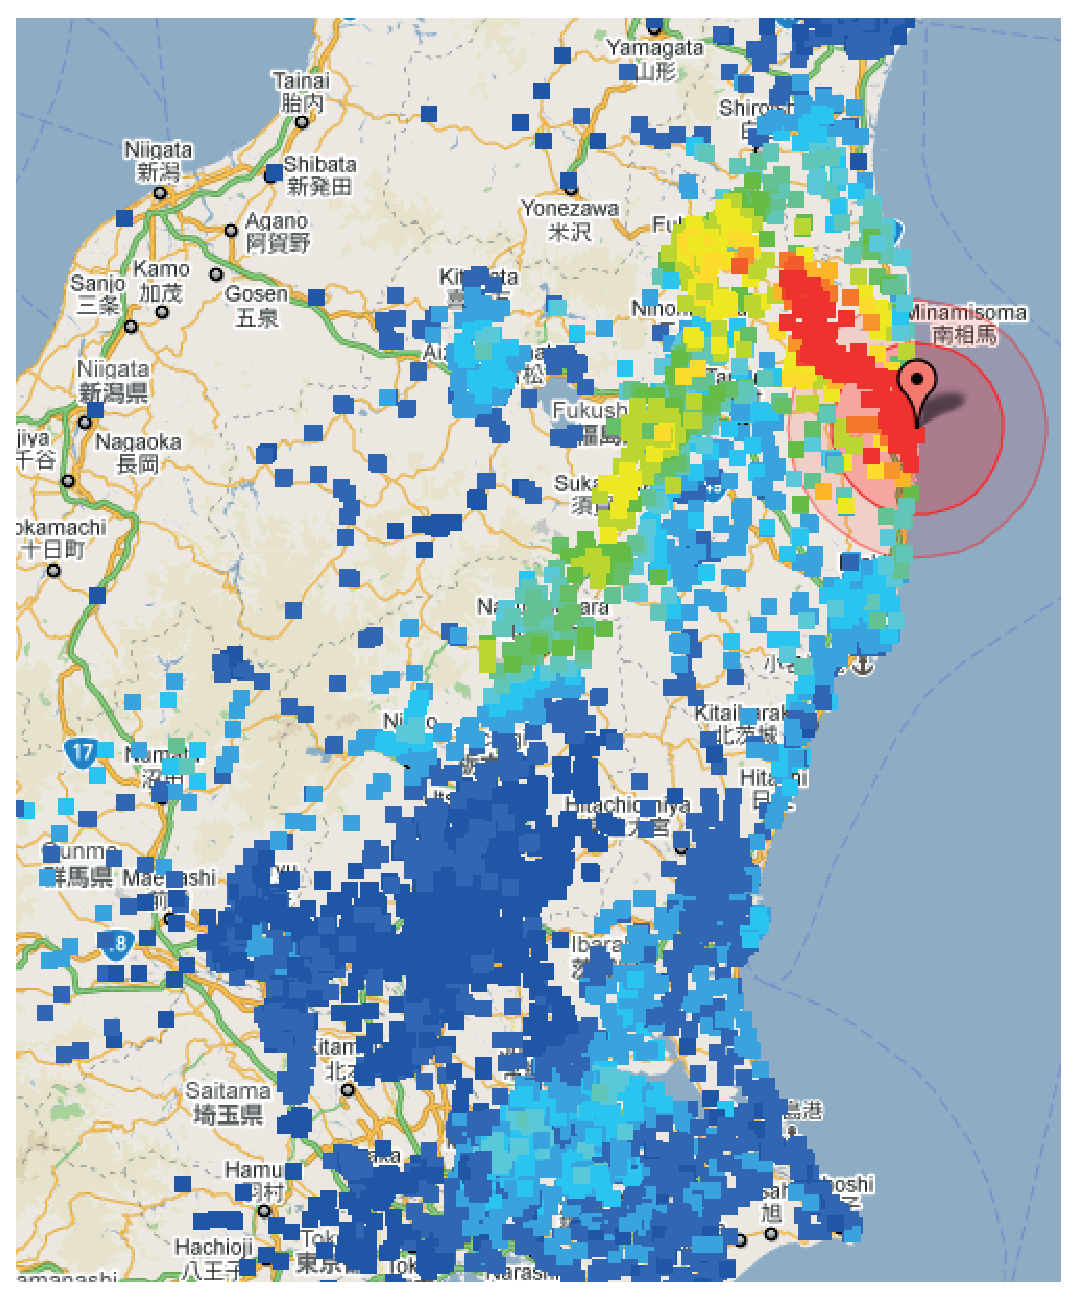
\includegraphics[width=\textwidth]{fukushima_1.eps}
%                \caption{Fukushima's environment radiation levels after nuclear disaster  \footnotemark}
%                \label{fig:fukushima_1}
%        \end{subfigure}
%        ~ %add desired spacing between images, e. g. ~, \quad, \qquad etc.
%          %(or a blank line to force the subfigure onto a new line)
%        \begin{subfigure}[t]{0.62\textwidth}
%                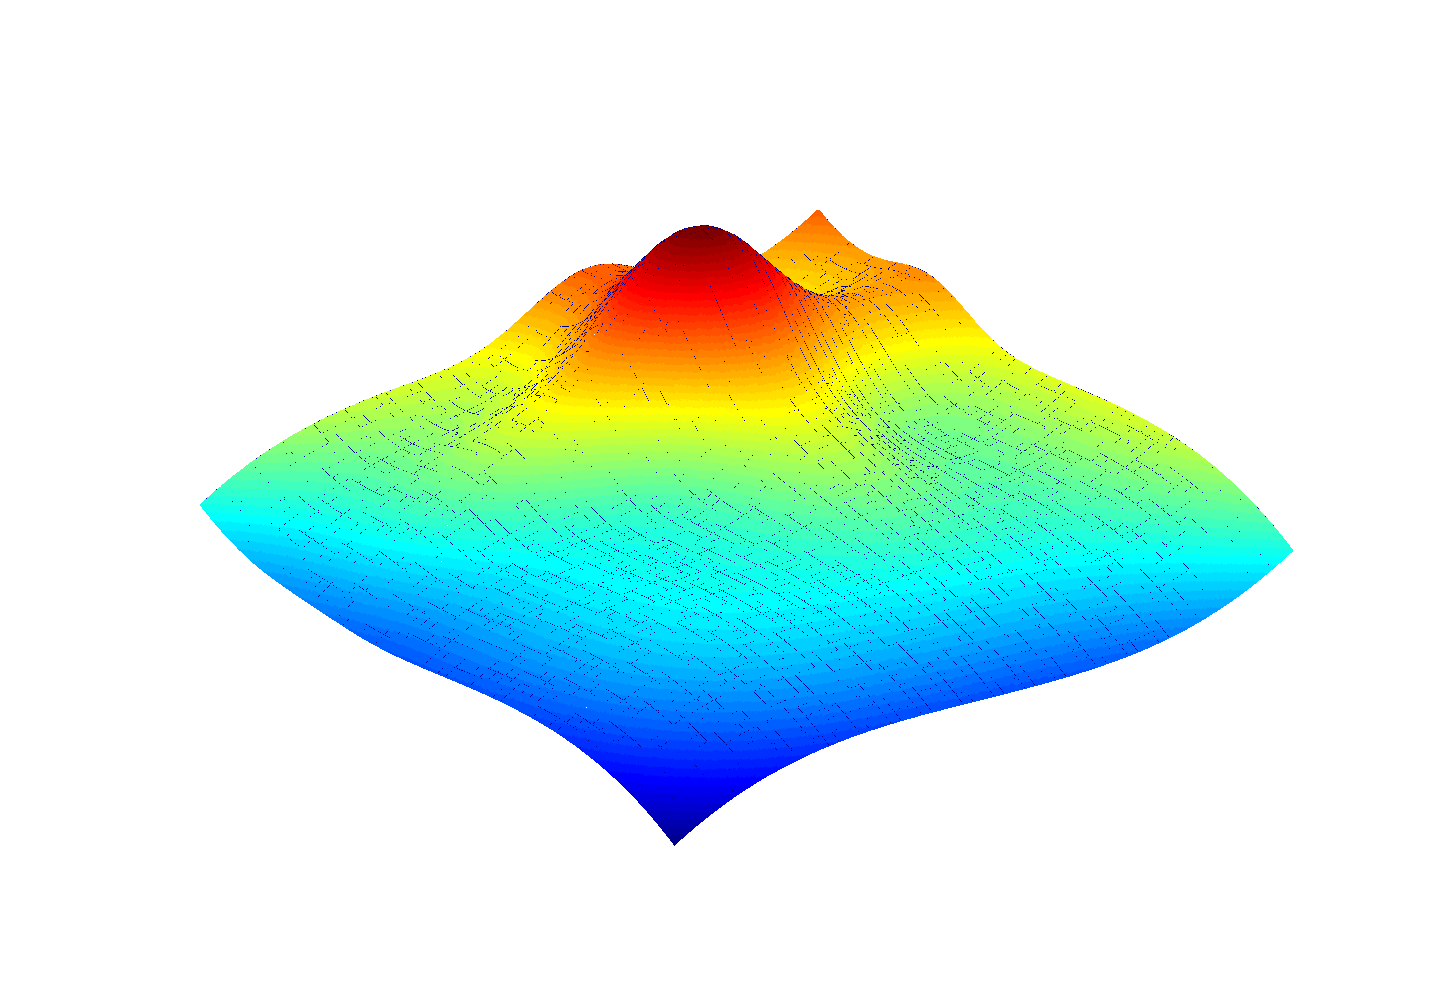
\includegraphics[width=\textwidth]{scalarfieldsource.eps}
%                \caption{Toxic cloud}
%                \label{fig:scalarfieldsource}
%        \end{subfigure}%
%        ~ %add desired spacing between images, e. g. ~, \quad, \qquad etc.
%          %(or a blank line to force the subfigure onto a new line)
%       \caption{Scalar fields} \label{fig:scalar field}
%\end{figure}
%\footnotetext[1]{Picture taken from FeedNetBack project}
%\footnotetext[2]{Picture taken from seaandskyjp.wordpress.com}
%}
% 



\chapter{Dynamic Model of the Quadrotor \label{ch:model}}

In this chapter, the dynamics of the quadrotor and the calculation of the mathematical model through two different approaches, are provided. In addition, the necessary considerations for the choice of a geometry configuration are exposed. This dynamic model and its inputs setting are needed to design the quadrotor flight controllers.
\\\\
Section \ref{sec:configurations} presents the description of two of the main used quadrotor geometry configurations. Also, this section presents what it means to choose one or the other configuration for the setting of the quadrotor inputs.
\\\\
The dynamic model of the quadrotor, obtained using the Newton-Euler and Euler-Lagrange approaches, neglecting the gyroscopic effects produced by the propellers, is shown in Section \ref{sec:nonlinear}.
\\\\
Finally, Section \ref{sec:linearized} describes an overview of the Jacobian linearization method applied to the quadrotor dynamic model and the thrust compensation needed to be implemented in a real quadrotor.

\section{Quadrotors Configurations}
\label{sec:configurations}
The term `quadrotor' refers to a rotary-wing UAV which thrust is generated using four motors and propellers. Quadrotors can be build in multiple ways.
There are two basic configurations which are widely used by commercial manufacturers and hobbyists. These two configurations are the `+' and the `X'.
%\\\\
%\url{https://www.google.com/search?q=why+\%2B+or+x+configuration+quadcopter&ie=utf-8&oe=utf-8&client=firefox-b-ab&gfe_rd=cr&dcr=0&ei=Mr0BWrW9HtHk8AfXm7fADQ}
%\\\\
%\url{https://community.micro-motor-warehouse.com/t/vs-x-configuration/2673}
%\\\\
%\url{https://www.quora.com/Why-is-x-configuration-preferred-over-+-config-of-quadcopter}
%\\\\
%\url{https://www.rcgroups.com/forums/showthread.php?1203569-Quad-X-vs-configuration}


\subsection{The `+' Configuration}
The geometry used in quadrotors built in `+' configuration is shown in Fig. \ref{fig:quadcopterplus}.
\\
\begin{figure}[H]
\begin{center}
  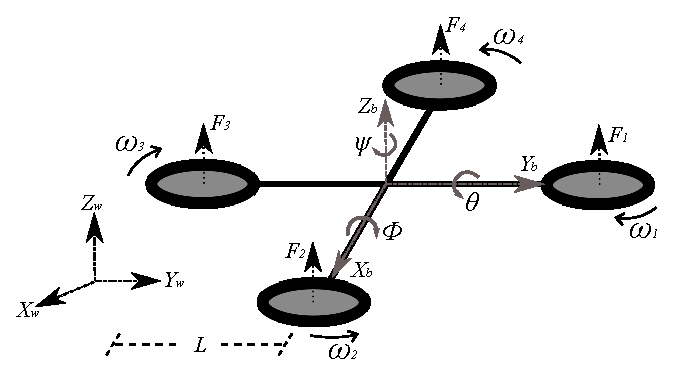
\includegraphics[width=0.90\textwidth]{quadcopterplus.eps}
\caption{Quadrotor geometry in `+' configuration} 
    \label{fig:quadcopterplus}
    \end{center}
\end{figure}
In Fig. \ref{fig:quadcopterplus}, ($\phi$, $\theta$, $\psi$) are the angular deviations (pitch, roll and yaw, respectively) of the quadrotor about the body-frame;
 ($x$, $y$, $z$) are the body-frame axes;  ($X_W$, $Y_W$, $Z_W$) are the earth-frame axes; $L$ is the distance from the quadrotor center of gravity ($CoG$) to the motors center; $F_{M_i}$ is the thrust force exerted by each motor $M_i$; and $\omega_i$ is the angular velocity of $M_i$, with $i = 1,2,3,4$. In this configuration, the body-frame axes $x$ and $y$, coincide with the lines that connect motors of opposite sides in the quadrotor frame.
\\\\
The quadrotor is a system with six $DoF$. Since a quadrotor has four actuators, it can be considered an underactuated system. This means that, it is only possible to reach a desired state for four $DoF$. However, it is possible to indirectly control the two remaining $DoF$ choosing the control signals appropriately. These control signals, or inputs, represent the quadrotor basic movements and are described below.

\begin{itemize}
\item \textbf{Thrust $T_u$ [$N$]}\\\\
The thrust $T_u$ is the total thrust force exerted parallel to the body-frame $z$-axis by the four motors. This thrust, can also generate accelerations in the direction of the $X_W$ and $Y_W$ axes. This happens when $|\theta| > 0$ or $|\phi| > 0$.
\\\\
This control signal affects the speed of rotation of all motors, and therefore their thrust, in equal magnitude, and is set as
\begin{equation}
\label{ec:u+}
T_u = \sum_{i=1}^{4}F_{M_i}.
\end{equation}

\item \textbf{Yaw Torque $\tau_{\psi}$ [$N\cdot m$]}\\\\
From Fig. \ref{fig:quadcopterplus}, $M_1$ and $M_3$ have a clockwise ($CW$) rotation while $M_2$ and $M_4$ rotate counter-clockwise ($CCW$). This configuration of opposite pairs rotational directions allows the system to control its conservation of momentum, and thus change its yaw angle in a controlled manner. This is done unbalancing the total momentum around the $z$-axis and without the need of a tail rotor used in the standard helicopter structure (\cite{Bresciani2008}). In `+' configuration, the fact that the pitch and roll angles are controlled using only two motors that rotate in the same direction, leads to large changes in the thrust force of the other two motors to achieve conservation of momentum.
\\\\
This conservation of momentum is controlled using the torque generated by each motor ($\tau_{M_i}$) around the body-frame $z$-axis. It produces a turn in the opposite direction to the rotation of the motor. Taking into account that the torque $\tau_\psi$ is positive when it generates a clock-wise rotation around the $z$-axis, only $M_2$ and $M_4$ contribute positively to it. While the other tow motors have a negative contribution to $\tau_\psi$. Thus, the total torque around the $z$-axis is depicted as
\begin{equation}
\label{ec:taupsiTM}
\tau_{\psi} = \tau_{M_2} + \tau_{M_4} - \tau_{M_1} - \tau_{M_3}.
\end{equation}
Each torque $\tau_{M_i}$ has a linear relationship with the thrust applied by the motor, with $K_M$ being the proportional constant and
\begin{equation}
\label{ec:taumi}
\tau_{M_{i}} = K_{M}F_{M_i}.
\end{equation}
Replacing (\ref{ec:taumi}) in (\ref{ec:taupsiTM}) the total torque $\tau_\psi$ dependence on the forces $F_{M_i}$ is got as
\begin{equation}
\label{ec:taupsi+}
\tau_{\psi} = K_{m}(F_{M_2} + F_{M_4} - F_{M_1} - F_{M_3}).
\end{equation}

\item \textbf{Roll Torque $\tau_{\theta}$ [$N\cdot m$]}\\\\
The roll torque $\tau_\theta$ is described as the torque exerted on the $x$-axis and about the $y$-axis. In the `+' configuration, the only motors that affect the quadrotor rotation with respect to the $x$-axis are $M_2$ and $M_4$. These do not affect the rotation with respect to the $y$-axis. In this case, the torques are generated by the forces $F_{M_2}$ and $F_{M_4}$ being applied at a distance $L$ from the quadrotor $CoG$. Considering a positive $\tau_\theta$ as the one causing a counter clock-wise rotation about the $y$-axis, the roll torque in `+' is set as
\begin{equation}
\label{ec:tautheta+}
\tau_{\theta} = L(F_{M_4}-F_{M_2}).
\end{equation}

\item \textbf{Pitch Torque $\tau_{\phi}$ [$N\cdot m$]}\\\\
Unlike the roll torque, the pitch torque $\tau_\phi$ is the one exerted on the $y$-axis about the $x$-axis. As Fig. \ref{fig:quadcopterplus} shows, $M_1$ and $M_3$ are the motors applying the forces that create this torque. Being $\tau_\phi$ positive when clock-wise rotation about the $x$-axis is caused, it is defined for a `+' configuration as
\begin{equation}
\label{ec:tauphi+}
\tau_{\phi} = L(F_{M_3}-F_{M_1}).
\end{equation}
\end{itemize}

\subsubsection{Inputs Setting in `+' Configuration}
Summarizing, the `+' configuration quadrotor inputs are established as linear combinations of the motors forces $F_{M_i}$. Equations (\ref{ec:u+}), (\ref{ec:taupsi+}), (\ref{ec:tautheta+}) and (\ref{ec:tauphi+}) integrate a linear equations system where the vector of inputs $\mathbf{u_{(+)}}$ is
\begin{equation}
	\mathbf{u_{(+)}} = \begin{bmatrix}
	T_u\\[5pt]
	\tau_{\psi}\\[5pt]
	\tau_{\theta}\\[5pt]
	\tau_{\phi}
	\end{bmatrix} = \begin{bmatrix}
	1 & 1 & 1 & 1 \\[5pt]
	-K_{m} & K_{m} & -K_{m} & K_{m}\\[5pt]
	0 & -L & 0 & L\\[5pt]
	-L & 0 & L & 0
							\end{bmatrix}
\begin{bmatrix}
F_{M_1}\\[5pt]
F_{M_2}\\[5pt]
F_{M_3}\\[5pt]
F_{M_4}
\end{bmatrix}.
	\label{ec:U_+}						
\end{equation}

\subsection{The `X' Configuration}
Following the same nomenclature used in the `+' configuration, in `X' configuration, the quadrotor frame is rotated $\pi/4\ rad$ about the $z$-axis in the body-frame, as shown in Fig. \ref{fig:quadrotorX}. 
\\\\
In this case, the front-line in the quadrotor is set between $M_1$ and $M_4$. In `X' configuration, the roll and pitch torques are applied using the forces exerted by all the motors at a distance $L_X = L\cdot \cos(\pi/4)$ (\cite{Faessler2016}).  This geometry is shown in Fig. \ref{fig:quadrotorX}.
\begin{figure}[H]
\begin{center}
  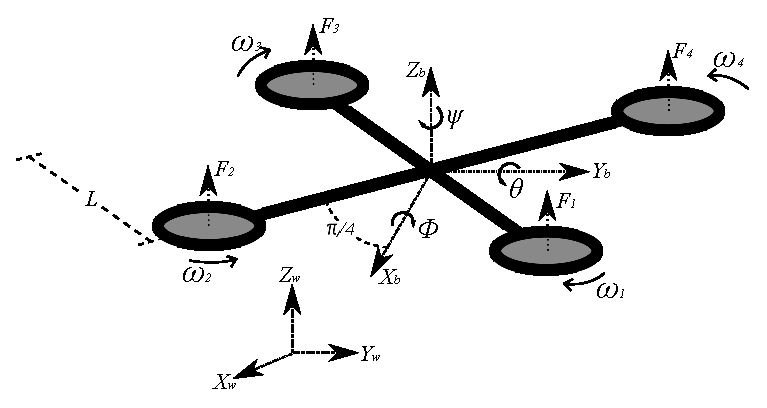
\includegraphics[width=0.97\textwidth]{quadcopter1.eps}
% figure caption is below the figure
\caption{Quadrotor geometry in `X' configuration} 
    \label{fig:quadrotorX}
    \end{center}
\end{figure}
The inputs description for the quadrotor `X' configuration is defined as follows.
\begin{itemize}
\item \textbf{Thrust $T_u$ [$N$]}\\\\
The total thrust exerted by the four motors in the quadrotor is not changed between the `+' and `X' configurations. Hence, the thrust $T_u$ is defined as
\begin{equation}
\label{ec:ux}
T_u = \sum_{i=1}^{4}F_{M_i}.
\end{equation}

\item \textbf{Yaw Torque $\tau_{\psi}$ [$N\cdot m$]}\\\\
As the $z$-axis is not modified between the `+' and `X' configurations, and the motors rotate in the same direction as in the other configuration, the yaw torque $\tau_\psi$ is set as
\begin{equation}
\label{ec:taupsix}
\tau_{\psi} = K_{m}(F_{M_2} + F_{M_4} - F_{M_1} - F_{M_3}).
\end{equation}
\\\\
\item \textbf{Roll Torque $\tau_{\theta}$ [$N\cdot m$]}\\\\
As shown in Fig. \ref{fig:quadrotorX}, roll and pitch torques are affected by the effects of all the quadrotor motors. For the roll torque $\tau_{\theta}$, the motors $M_3$ and $M_4$ contribute positively, while $M_1$ and $M_2$ have a negative contribution to it. In this case, the roll torque is depicted as
\begin{equation}
\label{ec:tauthetax}
\tau_{\theta} = L_{X}(F_{M_3}+F_{M_4}-F_{M_2}-F_{M_1}).
\end{equation}

\item \textbf{Pitch Torque $\tau_{\phi}$ [$N\cdot m$]}\\\\
Due to the $CW$ positive direction of the $\phi$ angle, and considering the sign of the contribution exerted by each force $F_{M_i}$, the pitch torque for the `X' configuration is defined as
\begin{equation}
\label{ec:tauphix}
\tau_{\phi} = L_{X}(F_{M_2}+F_{M_3}-F_{M_1}-F_{M_4}).
\end{equation}

\end{itemize}

\subsubsection{Inputs Setting in `X' Configuration}
In the `X' configuration, the quadrotor inputs remain the same regarding the `+' configuration. However both $\tau_\theta$ and $\tau_\phi$ are affected by the interaction of all the motors and the change in the distance of the point of application of the forces $F_{M_i}$ on the $x$ and $y$ axes. The linear equations system that shows the inputs setting for a quadrotor in `X' configuration is defined as
\begin{equation}
	\mathbf{u_{(X)}} = \begin{bmatrix}
	T_u\\[5pt]
	\tau_{\psi}\\[5pt]
	\tau_{\theta}\\[5pt]
	\tau_{\phi}
	\end{bmatrix} = \begin{bmatrix}
	1 & 1 & 1 & 1 \\[5pt]
	-K_{m} & K_{m} & -K_{m} & K_{m}\\[5pt]
	-L_{X} & -L_{X} & L_{X} & L_{X}\\[5pt]
	-L_{X} & L_{X} & L_{X} & -L_{X}
							\end{bmatrix}
\begin{bmatrix}
F_{M_1}\\[5pt]
F_{M_2}\\[5pt]
F_{M_3}\\[5pt]
F_{M_4}
\end{bmatrix}.
	\label{ec:U_X}						
\end{equation}

\subsubsection{Maximum Torque About $x$ and $y$ axes in `X' Configuration}
In `+' configuration, the torques around the $x$ and $y$ axes are set using just two motors applying a force at a distance $L$ from the quadrotor $CoG$. This implies that, for instance, in the case of roll torque $\tau_\theta$ the maximum torque $\tau_{\theta max (+)}$ is achieved when $F_{M_4} = F_{M_i max}$ and $F_{M_3} = 0$, where $F_{M_i max}$ is the maximum thrust of the motors. Then, in `+' configuration, the $\tau_{\theta max (+)}$ is set as
\begin{equation}
\tau_{\theta max (+)} = L\cdot F_{M_i max}
\end{equation}
On the other hand, the torques around the $x$ and $y$ axes in `X' configuration depend on the forces of the four motors in the quadrotor, which are applied at a distance $L_{X} = L\cdot \cos(\pi/4)$ from the quadrotor $CoG$. Continuing with the example of the roll torque, in `X' configuration the maximum torque $\tau_{\theta max (X)}$ is achieved when $F_{M_3} = F_{M_4} = F_{M_i max}$ and $F_{M_1} = F_{M_2} = 0$. Hence, the maximum torque about the $y$-axis in `X' configuration is
\begin{align}
\begin{split}
\tau_{\theta max (X)} & = L\cdot \cos(\pi/4) \cdot 2 \cdot F_{M_i max}\\[5px]
\tau_{\theta max (X)} & = 2\cdot \cos(\pi/4) \cdot \tau_{\theta max (+)}\\[5px]
\end{split}
\end{align}
Thereby, the quadrotor in `X' configuration has $2\cdot \cos(\pi/4)$ times more available torque to rotate about the $x$ and $y$ axes, when compared with the `+' configuration, and therefore it can achieve $41.42\ \%$ more rotational acceleration about the $x$ and $y$ axes.


\section{Non-linear Model}
\label{sec:nonlinear}

This section describes the dynamic modeling used to develop the quadrotor control, based on the study carried out in \cite{Bresciani2008} and \cite{Bouabdallah2007}. This model represents the quadrotor as a solid symmetrical object, subject to a total thrust ($T_u$) and three torques ($\tau_\psi$, $\tau_\theta$ and $\tau_\phi$), assuming that the quadrotor $CoG$ coincides with the origin of the body-frame and without considering the dynamics of the actuators . The modeling of the quadrotor system is done by two different methods. The Newton-Euler approach is based on the quadrotor body-frame, while the Euler-Lagrange approach bases its translational equations in the earth-frame while keeping its rotational equations related to the body-frame.

\subsection{Newton-Euler Approach}
Following the quadrotor geometry shown in Fig. \ref{fig:quadrotorX}, the quadrotor position vector ($\mathbf{\Xi}$), composed by the translational position ($\mathbf{\Gamma_W}$ [$m$]) and rotational position ($\mathbf{\Theta_W}$ [$rad$]) regarding the earth-frame, is defined as
\begin{equation}
\mathbf{\Xi} = \begin{bmatrix}
\mathbf{\Gamma_W} \\ \mathbf{\Theta_W}
\end{bmatrix} = \begin{bmatrix}
X_W \\ Y_W \\ Z_W \\ \psi \\ \theta \\ \phi
\end{bmatrix}.
\end{equation}
On the other hand, the quadrotor velocity vector ($\mathbf{\nu}$) is composed by the translational ($\mathbf{V_B}$ [$m\cdot s^{-1}$]) and rotational ($\mathbf{\Omega_B}$ [$rad\cdot s^{-1}$]) velocities with respect to the body-frame as
\begin{equation}
\mathbf{\nu} = \begin{bmatrix}
\mathbf{V_B} \\ \mathbf{\Omega_B}
\end{bmatrix} =
\begin{bmatrix}
\dot{x} \\ \dot{y} \\ \dot{z} \\ \dot{\psi} \\ \dot{\theta} \\ \dot{\phi}
\end{bmatrix}.
\end{equation}
Therefore exists a generalized matrix
\begin{equation}
\mathbf{\zeta_\Theta} = \begin{bmatrix}
\mathbf{R_{b}^{w}} & \mathbf{0_{3\times 3}} \\
\mathbf{0_{3\times 3}} & \mathbf{T_{b}^{w}}
\end{bmatrix},
\end{equation}
that ensures that
\begin{equation}
\mathbf{\dot{\Xi}} = \mathbf{\zeta_\Theta}\mathbf{\nu},
\end{equation}
where $\mathbf{0_{3\times 3}}$ is a $3\times 3$-matrix filled with zeros, $\mathbf{R_{b}^{w}}$ is the rotation matrix and $\mathbf{T_{b}^{w}}$ the transfer matrix from the body to the world-frame, defined as
\begin{equation}
\mathbf{R_{b}^{w}} = \begin{bmatrix}
c_\theta c_\psi & c_\psi s_\theta s_\phi-c_\phi s_\psi & s_\phi s_\psi+c_\phi c_\psi s_\theta\\
c_\theta s_\psi & s_\psi s_\theta s_\phi+c_\phi c_\psi & c_\phi s_\psi s_\theta - s_\phi c_\psi\\
-s_\theta & c_\theta s_\phi & c_\theta c_\phi
\end{bmatrix},
\end{equation}
\begin{equation}
\mathbf{T_{b}^{w}} = \begin{bmatrix}
1 & s_\phi t_\theta & c_\phi t_\theta\\
0 & c_\phi & -s_\phi\\
0 & s_\phi / c_\theta & c_\phi / c_\theta 
\end{bmatrix},
\end{equation}
with $s_\theta = \sin(\theta)$, $c_\theta = \cos(\theta)$, and $t_\theta = \tan(\theta)$.
\\\\
As the quadrotor is assumed to be a rigid body of 6 $DoF$, its dynamics consider the mass ($m$ [$kg$]) and the inertia matrix ($\mathbf{J}$ [$kg\cdot m^{2}$]) of it, and are described as
\begin{equation}
\label{eqn:eomNewtonEuler}
\mathbf{M_{B}}\mathbf{\dot{\nu}} + \mathbf{S_\nu} = \mathbf{\Lambda}
\end{equation}
where
\begin{align}
\begin{split}
\mathbf{M_{B}} & = \begin{bmatrix}
m\mathbf{I_{3\times3}} & \mathbf{0_{3\times 3}} \\
\mathbf{0_{3\times 3}} & \mathbf{J}
\end{bmatrix} = \begin{bmatrix}
m & 0 & 0 & 0 & 0 & 0 \\
0 & m & 0 & 0 & 0 & 0 \\
0 & 0 & m & 0 & 0 & 0 \\
0 & 0 & 0 & J_{zz} & 0 & 0 \\
0 & 0 & 0 & 0 & J_{yy} & 0 \\
0 & 0 & 0 & 0 & 0 & J_{xx}
\end{bmatrix},\\[8px]
\dot{\nu} & = \begin{bmatrix}
\mathbf{\dot{V}_{B}} \\ \mathbf{\dot{\Omega}_B}
\end{bmatrix}, \\[8px]
\mathbf{S_\nu} & = \begin{bmatrix}
\mathbf{\Omega_B} \times m\mathbf{V_{B}} \\
\mathbf{\Omega_B} \times \mathbf{J}\mathbf{\Omega_B}
\end{bmatrix} =
\begin{bmatrix}
m(\ddot{x} + \dot{z}\dot{\theta} - \dot{y}\dot{\phi})\\
m(\ddot{y} + \dot{x}\dot{\phi} - \dot{z}\dot{\psi})\\
m(\ddot{z} + \dot{y}\dot{\psi} - \dot{x}\dot{\theta})\\
J_{zz}\dot{\psi} + \dot{\theta}\dot{\phi}(J_{xx} - J_{yy})\\
J_{yy}\dot{\theta} + \dot{\psi}\dot{\phi}(J_{zz} - J_{xx})\\
J_{xx}\dot{\phi} + \dot{\psi}\dot{\theta}(J_{yy} - J_{zz})\\
\end{bmatrix},\\[8px]
\mathbf{\Lambda} & = \begin{bmatrix}
\mathbf{F_{B}} \\ \mathbf{\tau_{B}}
\end{bmatrix} = \begin{bmatrix}
F_x & F_y & F_z & \tau_z & \tau_y & \tau_x
\end{bmatrix}^{T},
\end{split}
\end{align}
being $\mathbf{J}$ diagonal due to the assumption of a perfect symmetric quadrotor body, $\mathbf{I}$ the identity matrix, $\mathbf{\dot{V}_{B}}$ is the quadrotor translational acceleration in the body-frame, $\mathbf{\dot{\Omega}_B}$ is the quadrotor angular acceleration in the body-frame, $\mathbf{F_{B}}$ is the quadrotor force vector and $\mathbf{\tau_{B}}$ is the quadrotor torques vector.
\\\\
The forces and torques vector $\mathbf{\Lambda}$ results from the effect of the gravitational force (represented in $\mathbf{G_{\Lambda}}$), the quadrotor inputs created by the motor forces (represented in $\mathbf{U_{\Lambda}}$), and the gyroscopic effects produced when the motors propellers are rotating (represented in $\mathbf{P_{\Lambda}}$). However in this project, for simplicity in the dynamic model, it is not taken into account the $\mathbf{P_{\Lambda}}$ contribution to the $\mathbf{\Lambda}$ vector and thus $\mathbf{P_{\Lambda}} \approx \mathbf{0_{6\times 1}}$.
\\\\
The gravitational force affects just the $\mathbf{F_B}$ component in $\mathbf{\Lambda}$, proportionally to its magnitude $|\vec{g}|= g = 9.807\ m/s^{2}$. $\mathbf{G_{\Lambda}}$ is the contribution of the gravitational force to the vector $\mathbf{\Lambda}$ and is expressed as 
\begin{equation}
\mathbf{G_{\Lambda}}= \begin{bmatrix}
\mathbf{\hat{F}_{Gb}} \\ \mathbf{0_{3\times 1}}
\end{bmatrix} = \begin{bmatrix}
\mathbf{R_{b}^{w}}\mathbf{F_{G\xi}} \\ \mathbf{0_{3\times 1}}
\end{bmatrix} = 
\begin{bmatrix}
\mathbf{R_{w}^{b}} 
\begin{bmatrix}
0 \\[5pt] 0 \\[5pt] -m g
\end{bmatrix} \\[5pt]
\mathbf{0_{3\times 1}}
\end{bmatrix} =\begin{bmatrix}
m g \sin(\theta) \\[5pt]
m g \cos(\theta)\sin(\phi) \\[5pt]
- m g \cos(\theta)\sin(\phi) \\[5pt]
\mathbf{0_{3\times 1}}
\end{bmatrix}
\end{equation}
were $\mathbf{F_{G\xi}}=\mathbf{R_{b}^{w}}\mathbf{\hat{F}_{Gb}}$ is the translational force due to  gravity in the earth-frame, and $\mathbf{R_{w}^{b}} = (\mathbf{R_{b}^{w})^{-1}}$ is the rotation matrix from the world to the body-frame.
\\\\
From Section \ref{sec:configurations}, it follows that the quadrotor inputs are proportional to the motor forces $F_{M_i}$, and do not affect the $x$ and $y$ components of $\mathbf{F_B}$. These inputs, depend on the quadrotor configuration (`+' or `X') and are set as
\begin{equation}
\mathbf{u_{\Lambda}} = \begin{bmatrix}
0 \\[5pt] 0 \\[5pt] u_1 \\[5pt] u_2 \\[5pt] u_3 \\[5pt] u_4
\end{bmatrix} = \begin{bmatrix}
0 \\[5pt] 0 \\[5pt] T_u\\[5pt]
	\tau_{\psi}\\[5pt]
	\tau_{\theta}\\[5pt]
	\tau_{\phi}
\end{bmatrix}
\end{equation}
where $T_u$, $\tau_\psi$, $\tau_\theta$ and $\tau_\phi$ depend on the configuration of the quadrotor as exposed in (\ref{ec:U_+}) and (\ref{ec:U_X}).
\\\\
Thus, (\ref{eqn:eomNewtonEuler}) can be redefined as
\begin{equation}
\label{eqn:eomNewtonEulerfull}
\mathbf{M_{B}}\mathbf{\dot{\nu}} + \mathbf{S_\nu} = \mathbf{G_{\Lambda}} + \mathbf{u_{\Lambda}}.
\end{equation}
The quadrotor acceleration vector $\mathbf{\dot{\nu}}$ in the body-frame is then isolated from (\ref{eqn:eomNewtonEulerfull}), getting
\begin{equation}
\mathbf{\dot{\nu}} = \mathbf{M_{B}}^{-1}(-\mathbf{S_\nu} + \mathbf{G_{\Lambda}} + \mathbf{u_{\Lambda}}),
\end{equation}
or expressed as a system of equations
\begin{align}
\begin{split}
\ddot{x} & = \dot{y} \dot{\phi} - \dot{z} \dot{\theta} + g \sin(\theta), \\[5pt]
\ddot{y} & = \dot{z} \dot{\psi} - \dot{x} \dot{\phi} + g \cos(\theta)\sin(\phi), \\[5pt]
\ddot{z} & = \dot{x} \dot{\theta} - \dot{y} \dot{\psi} - g \sin(\theta) + \dfrac{u_{1}}{m}, \\[5pt]
\ddot{\psi} & = \dot{\phi}\dot{\theta} \dfrac{J_{xx}-J_{yy}}{J_{zz}} + \dfrac{u_{2}}{J_{zz}}, \\[5pt]
\ddot{\theta} & = \dot{\phi} \dot{\psi}\dfrac{J_{zz}-J_{xx}}{J_{yy}} + \dfrac{u_{3}}{J_{yy}}, \\[5pt]
\ddot{\phi} & =  \dot{\theta}\dot{\psi}\dfrac{J_{yy}-J_{zz}}{J_{xx}} + \dfrac{u_{4}}{J_{xx}},
\end{split}
\end{align}
with the inputs set as
\begin{equation}
\begin{bmatrix}
u_1 \\[5pt] u_2 \\[5pt] u_3 \\[5pt] u_4
\end{bmatrix} = \begin{bmatrix}
	T_u\\[5pt]
	\tau_{\psi}\\[5pt]
	\tau_{\theta}\\[5pt]
	\tau_{\phi}
	\end{bmatrix} = \begin{bmatrix}
	1 & 1 & 1 & 1 \\[5pt]
	-K_{m} & K_{m} & -K_{m} & K_{m}\\[5pt]
	0 & -L & 0 & L\\[5pt]
	-L & 0 & L & 0
							\end{bmatrix}
\begin{bmatrix}
F_{M_1}\\[5pt]
F_{M_2}\\[5pt]
F_{M_3}\\[5pt]
F_{M_4}
\end{bmatrix}					
\end{equation}
for quadrotors in `+' configuration, and
\begin{equation}
\begin{bmatrix}
u_1 \\[5pt] u_2 \\[5pt] u_3 \\[5pt] u_4
\end{bmatrix}	 = \begin{bmatrix}
	T_u\\[5pt]
	\tau_{\psi}\\[5pt]
	\tau_{\theta}\\[5pt]
	\tau_{\phi}
	\end{bmatrix} = \begin{bmatrix}
	1 & 1 & 1 & 1 \\[5pt]
	-K_{m} & K_{m} & -K_{m} & K_{m}\\[5pt]
	-L_{X} & -L_{X} & L_{X} & L_{X}\\[5pt]
	-L_{X} & L_{X} & L_{X} & -L_{X}
							\end{bmatrix}
\begin{bmatrix}
F_{M_1}\\[5pt]
F_{M_2}\\[5pt]
F_{M_3}\\[5pt]
F_{M_4}
\end{bmatrix}
\end{equation}
for quadrotors in `X' configuration.
\\\\
Defining the state vector as
\setcounter{MaxMatrixCols}{20}
\begin{equation}
\mathbf{x} = \begin{bmatrix}
x & \dot{x} & y & \dot{y} & z & \dot{z} & \psi & \dot{\psi} & \theta & \dot{\theta} & \phi & \dot{\phi}
\end{bmatrix}^{T},
\end{equation} 
the quadrotor non-linear dynamics model $\mathbf{f(x,u)}$ got with a Newton-Euler approach is
\begin{equation}
\mathbf{\dot{x}} = \mathbf{f(x,u)} = \begin{bmatrix}
\dot{x} \\[5pt]
\dot{y} \dot{\phi} - \dot{z} \dot{\theta} + g \sin(\theta) \\[5pt]
\dot{y} \\[5pt]
\dot{z} \dot{\psi} - \dot{x} \dot{\phi} + g \cos(\theta)\sin(\phi) \\[5pt]
\dot{z} \\[5pt]
\dot{x} \dot{\theta} - \dot{y} \dot{\psi} - g \sin(\theta) + \dfrac{u_{1}}{m} \\[5pt]
\dot{\psi} \\[5pt]
\dot{\phi}\dot{\theta} \dfrac{J_{xx}-J_{yy}}{J_{zz}} + \dfrac{u_{2}}{J_{zz}} \\[5pt]
\dot{\theta} \\[5pt]
\dot{\phi} \dot{\psi}\dfrac{J_{zz}-J_{xx}}{J_{yy}} + \dfrac{u_{3}}{J_{yy}} \\[5pt]
\dot{\phi} \\[5pt]
\dot{\theta}\dot{\psi}\dfrac{J_{yy}-J_{zz}}{J_{xx}} + \dfrac{u_{4}}{J_{xx}}
\end{bmatrix}
\end{equation}

\subsection{Euler-Lagrange Approach}
The general coordinates representing the position and attitude of the quadrotor are defined as
\begin{equation}
	\mathbf{\Xi}=\begin{bmatrix}
	\mathbf{\xi_W} & \mathbf{\Theta_B}
	\end{bmatrix}^{T},
	\label{ec:coorgenerales}
\end{equation}
where $\mathbf{\xi_W}=\begin{bmatrix}
X_W & Y_W & Z_W
\end{bmatrix}^{T}$ is the vector representing the position of the $CoG$ of the quadrotor relative to the earth-frame shown in Fig. \ref{fig:quadrotorX} and $\mathbf{\Theta_B}=\begin{bmatrix}
\psi & \theta & \phi
\end{bmatrix}^{T}$ represent the quadrotor attitude.
\\\\
The Lagrangian of the quadrotor is defined by
\begin{equation}
	L(\mathbf{\Xi},\mathbf{\dot{\Xi}})=K_{trans}+K_{rot} - E_{pot},	
	\label{ec:lagrangiano}
\end{equation}
where $ K_{trans}$ is the quadrotor translational kinetic energy, $ K_{rot}$ is the quadrotor rotational kinetic energy, $E_{pot}$ is the quadrotor potential energy, and $z$ is the quadrotor elevation. Hence, the Lagrangian in (\ref{ec:lagrangiano}) is rewritten as
\begin{equation}
	L(\mathbf{\Xi},\mathbf{\dot{\Xi}})=\dfrac{m}{2}\mathbf{\dot{\xi}_W}^{T}\mathbf{\dot{\xi}_W} + \dfrac{1}{2}\mathbf{\dot{\Theta}_B}^{T}J\mathbf{\dot{\Theta}_B} - mgz.
	\label{ec:lagrangiano2}
\end{equation}
The dynamic model of the quadrotor is derived from the Euler-Lagrange equation
\begin{equation}
	\dfrac{d}{dt}\dfrac{\partial L}{\partial \mathbf{\dot{\Xi}}}-\dfrac{\partial L}{\partial \mathbf{\Xi}}=
	\begin{bmatrix}
	F_{\xi}\\
	\tau
	\end{bmatrix},
	\label{ec:eulerlag}
 \end{equation} 
where $F_{\xi}=R_{b}^{w}\hat{F_{b}}$ is the translational force applied to the quadrotor by its four motors, and $\tau = \begin{bmatrix}
\tau_\psi & \tau_\theta & \tau_\phi
\end{bmatrix}^{T}$.
\\\\
In the quadrotor body-frame, the translational force $\hat{F_{b}}$ is only applied in the $z$-axis, and thus it is represented by
\begin{equation}
	\hat{F_{b}}=\begin{bmatrix}
	0\\
	0\\
	T_u
	\end{bmatrix} = \begin{bmatrix}
	0\\
	0\\
	\sum_{i=1}^{4}F_{M_i}
	\end{bmatrix}.
 \label{ec:fuerzas}
 \end{equation} 
The system of equations that represent the dynamics of the quadrotor got using the Euler-Lagrange approach (\ref{ec:eulerlag}) is
\begin{align}
\label{ec:eomEulerLagrange}
\begin{split}
\ddot{X}_W &= \frac{u_{1}}{m}(\cos(\phi)\sin(\theta)\cos(\psi) + \sin(\phi)\sin(\psi)), \\[5pt]
\ddot{Y}_W &= \frac{u_{1}}{m}(\cos(\phi)\sin(\theta)\sin(\psi) - \sin(\phi)\cos(\psi)), \\[5pt]
\ddot{Z}_W &= \frac{u_{1}}{m}(\cos(\phi)\cos(\theta)) - g, \\[5pt]
\ddot{\psi} & = \dot{\phi}\dot{\theta}\dfrac{J_{xx}-J_{yy}}{J_{zz}} + \dfrac{u_{2}}{J_{zz}}, \\[5pt]
\ddot{\theta} & = \dot{\phi}\dot{\psi}\dfrac{J_{zz}-J_{xx}}{J_{yy}} + \dfrac{u_{3}}{J_{yy}}, \\[5pt]
\ddot{\phi} & = \dot{\theta}\dot{\psi}\dfrac{J_{yy}-J_{zz}}{J_{xx}} +  \dfrac{u_{4}}{J_{xx}},
\end{split}
\end{align}
with the inputs set as
\begin{equation}
\begin{bmatrix}
u_1 \\[5pt] u_2 \\[5pt] u_3 \\[5pt] u_4
\end{bmatrix} = \begin{bmatrix}
	T_u\\[5pt]
	\tau_{\psi}\\[5pt]
	\tau_{\theta}\\[5pt]
	\tau_{\phi}
	\end{bmatrix} = \begin{bmatrix}
	1 & 1 & 1 & 1 \\[5pt]
	-K_{m} & K_{m} & -K_{m} & K_{m}\\[5pt]
	0 & -L & 0 & L\\[5pt]
	-L & 0 & L & 0
							\end{bmatrix}
\begin{bmatrix}
F_{M_1}\\[5pt]
F_{M_2}\\[5pt]
F_{M_3}\\[5pt]
F_{M_4}
\end{bmatrix}					
\end{equation}
for quadrotors in `+' configuration, and
\begin{equation}
\begin{bmatrix}
u_1 \\[5pt] u_2 \\[5pt] u_3 \\[5pt] u_4
\end{bmatrix}	 = \begin{bmatrix}
	T_u\\[5pt]
	\tau_{\psi}\\[5pt]
	\tau_{\theta}\\[5pt]
	\tau_{\phi}
	\end{bmatrix} = \begin{bmatrix}
	1 & 1 & 1 & 1 \\[5pt]
	-K_{m} & K_{m} & -K_{m} & K_{m}\\[5pt]
	-L_{X} & -L_{X} & L_{X} & L_{X}\\[5pt]
	-L_{X} & L_{X} & L_{X} & -L_{X}
							\end{bmatrix}
\begin{bmatrix}
F_{M_1}\\[5pt]
F_{M_2}\\[5pt]
F_{M_3}\\[5pt]
F_{M_4}
\end{bmatrix}
\end{equation}
for quadrotors in `X' configuration (\cite{Emam2016, Badr2016}).
\\\\
Defining the state vector as
\setcounter{MaxMatrixCols}{20}
\begin{equation}
\mathbf{x} = \begin{bmatrix}
X_W & \dot{X_W} & Y & \dot{Y_W} & Z_W & \dot{Z_W} & \psi & \dot{\psi} & \theta & \dot{\theta} & \phi & \dot{\phi}
\end{bmatrix}^{T},
\end{equation} 
the quadrotor non-linear dynamics model got with an Euler-Lagrange approach, can be represented as
\begin{equation}
\mathbf{\dot{x}} = \mathbf{f(x,u)} = \begin{bmatrix}
\dot{X}_W \\[5pt]
\dfrac{u_{1}}{m}(\cos(\phi)\sin(\theta)\cos(\psi) + \sin(\phi)\sin(\psi)) \\[5pt]
\dot{Y}_W \\[5pt]
\dfrac{u_{1}}{m}(\cos(\phi)\sin(\theta)\sin(\psi) - \sin(\phi)\cos(\psi)) \\[5pt]
\dot{Z}_W \\[5pt]
\dfrac{u_{1}}{m}(\cos(\phi)\cos(\theta)) - g \\[5pt]
\dot{\psi} \\[5pt]
\dot{\phi}\dot{\theta} \dfrac{J_{xx}-J_{yy}}{J_{zz}} + \dfrac{u_{2}}{J_{zz}} \\[5pt]
\dot{\theta} \\[5pt]
\dot{\phi} \dot{\psi}\dfrac{J_{zz}-J_{xx}}{J_{yy}} + \dfrac{u_{3}}{J_{yy}} \\[5pt]
\dot{\phi} \\[5pt]
\dot{\theta}\dot{\psi}\dfrac{J_{yy}-J_{zz}}{J_{xx}} + \dfrac{u_{4}}{J_{xx}}
\end{bmatrix}
\end{equation}

\section{Linearized Model}
\label{sec:linearized}
\setcounter{MaxMatrixCols}{20}
\subsection{Jacobian Linearization}
The linearization of a non-linear system is done about an equilibrium point $\overline{\mathbf{x}}$ achieved with a specific input called equilibrium input $\overline{\mathbf{u}}$  where $\mathbf{f(\overline{x},\overline{u})} \approx \mathbf{0}$. In the quadrotor, such an equilibrium point can be the hover state where $\mathbf{\Omega_B} \to \mathbf{0_{3\times 1}}$, $\mathbf{\dot{\Omega}_B} \to \mathbf{0_{3\times 1}}$, and $\mathbf{V_{B}} \to \mathbf{0_{3\times 1}}$. This is
\begin{align}
\label{ec:equilibrium}
\begin{split}
\overline{\mathbf{x}} & = \begin{bmatrix}
\overline{x} & \dot{\overline{x}} & \overline{y} & \dot{\overline{y}} & \overline{z} & \dot{\overline{z}} & \overline{\psi} & \dot{\overline{\psi}} & \overline{\theta} & \dot{\overline{\theta}} & \overline{\phi} & \dot{\overline{\phi}}
\end{bmatrix}^{T}\\
 & = \begin{bmatrix}
\overline{x} & 0 & \overline{y} & 0 & \overline{z} & 0 & 0 & 0 & 0 & 0 & 0 & 0
\end{bmatrix}^{T},
\end{split}
\end{align}
where $\overline{x}$, $\overline{y}$ and $\overline{z}$ define a constant desired position in the body and earth-frame. When the quadrotor state is near the equilibrium point, the body and earth frames are assumed to coincide and thus $\mathbf{\dot{\xi}_W}\to \mathbf{V_{B}}$, $X_W \to x$, $Y_W \to y$, and $Z_W \to z$ (\cite{Sabatino2015}).\\\\
The equilibrium point shown in \ref{ec:equilibrium}, is obtained using a constant input value $\overline{\mathbf{u}}$ where only the thrust that overcomes gravity is applied, as shown below.
\begin{equation}
\overline{\mathbf{u}} = \begin{bmatrix}
T_u & \tau_\psi & \tau_\theta & \tau_\phi
\end{bmatrix}^{T} = \begin{bmatrix}
mg & 0 & 0 & 0
\end{bmatrix}^{T}
\end{equation}
\\
The Jacobian linearization is based on the fact that if the quadrotor is not exactly at the equilibrium point, but close to it with a small deviation $\delta_{\mathbf{x}} = \mathbf{x} - \overline{\mathbf{x}}$, due to an input deviation $\delta_{\mathbf{u}}= \mathbf{u} - \overline{\mathbf{u}}$ \cite{RanjanVepa2016}. The non-linear system is represented by
\begin{equation}
\label{ec:deltajacobian}
\dot{\delta_{\mathbf{x}}} =  \mathbf{f(\overline{x}+\delta_{\mathbf{x}},\overline{u}}+\delta_{\mathbf{u}}).
\end{equation}
Using the first order Taylor polynomial from (\ref{ec:deltajacobian}) and considering that $\mathbf{f(\overline{x},\overline{u})} \approx \mathbf{0}$, the following expression is obtained.
\begin{equation}
\label{ec:linearizedsystem}
\dot{\delta_{\mathbf{x}}} \approx 
\frac{\partial f(\mathbf{x},\mathbf{u})}{\partial \mathbf{x}}\Bigr|_{\substack{\mathbf{x}=\overline{\mathbf{x}}\\\mathbf{u}=\overline{\mathbf{u}}}} \delta_{\mathbf{x}} + \frac{\partial f(\mathbf{x},\mathbf{u})}{\partial \mathbf{u}}\Bigr|_{\substack{\mathbf{x}=\overline{\mathbf{x}}\\\mathbf{u}=\overline{\mathbf{u}}}} \delta_{\mathbf{u}}
\end{equation}
The equation (\ref{ec:linearizedsystem}) describes a linear time-invariant representation of the non-linear dynamics of the quadrotor near an equilibrium point $\overline{\mathbf{x}}$ and with an input that tends to be $\overline{\mathbf{u}}$, which is established as a state space model
\begin{align}
\begin{split}
\dot{\mathbf{x}}(t) & = A\mathbf{x}(t)+B\mathbf{u}(t)
\end{split}
\end{align}
where
\begin{align}
\begin{split}
\mathbf{x} = & \begin{bmatrix}
x & \dot{x} & y & \dot{y} & z & \dot{z} & \psi & \dot{\psi} & \theta & \dot{\theta} & \phi & \dot{\phi}
\end{bmatrix}^{T},\\[15px]
\mathbf{u} = & \begin{bmatrix}
T_u & \tau_\psi & \tau_\theta & \tau_\phi
\end{bmatrix}^{T},\\[15px]
A  = \frac{\partial f(\mathbf{x},\mathbf{u})}{\partial \mathbf{x}}\Bigr|_{\substack{\mathbf{x}=\overline{\mathbf{x}}\\\mathbf{u}=\overline{\mathbf{u}}}} = & 
\begin{bmatrix}
0 & 1 & 0 & 0 & 0 & 0 & 0 & 0 & 0 & 0 & 0 & 0\\[2px]
0 & 0 & 0 & 0 & 0 & 0 & 0 & 0 & g & 0 & 0 & 0\\[2px]
0 & 0 & 0 & 1 & 0 & 0 & 0 & 0 & 0 & 0 & 0 & 0\\[2px]
0 & 0 & 0 & 0 & 0 & 0 & 0 & 0 & 0 & 0 & g & 0\\[2px]
0 & 0 & 0 & 0 & 0 & 1 & 0 & 0 & 0 & 0 & 0 & 0\\[2px]
0 & 0 & 0 & 0 & 0 & 0 & 0 & 0 & 0 & 0 & 0 & 0\\[2px]
0 & 0 & 0 & 0 & 0 & 0 & 0 & 1 & 0 & 0 & 0 & 0\\[2px]
0 & 0 & 0 & 0 & 0 & 0 & 0 & 0 & 0 & 0 & 0 & 0\\[2px]
0 & 0 & 0 & 0 & 0 & 0 & 0 & 0 & 0 & 1 & 0 & 0\\[2px]
0 & 0 & 0 & 0 & 0 & 0 & 0 & 0 & 0 & 0 & 0 & 0\\[2px]
0 & 0 & 0 & 0 & 0 & 0 & 0 & 0 & 0 & 0 & 0 & 1\\[2px]
0 & 0 & 0 & 0 & 0 & 0 & 0 & 0 & 0 & 0 & 0 & 0
\end{bmatrix}, \\[15px]
B = \frac{\partial f(\mathbf{x},\mathbf{u})}{\partial \mathbf{u}}\Bigr|_{\substack{\mathbf{x}=\overline{\mathbf{x}}\\\mathbf{u}=\overline{\mathbf{u}}}} = & 
\begin{bmatrix}
0 & 0 & 0 & 0 & 0 & \dfrac{1}{m} & 0 & 0 & 0 & 0 & 0 & 0\\[5px]
0 & 0 & 0 & 0 & 0 & 0 & 0 & \dfrac{1}{J_{zz}} & 0 & 0 & 0 & 0\\[5px]
0 & 0 & 0 & 0 & 0 & 0 & 0 & 0 & 0 & \dfrac{1}{J_{yy}} & 0 & 0\\[5px]
0 & 0 & 0 & 0 & 0 & 0 & 0 & 0 & 0 & 0 & 0 & \dfrac{1}{J_{xx}}
\end{bmatrix}^{T}.
\end{split}
\end{align}

\subsection{Thrust Compensation}
%\url{https://robotics.stackexchange.com/questions/4247/tilt-compensated-motor-output-to-keep-altitude-for-quadcopter}
Given the fact that the forces $F_{M_i}$ applied by the motors in the quadrotor are parallel to the body-frame $z$-axis and not to the earth-frame $Z_W$-axis, a compensated thrust input $u_{1}^{*}$ must be set so that its projection $u_1$ (third component of $F_\xi$) on the $Z_W$-axis is such that it allows to keep the inputs of the system close to the equilibrium input, even though there are deviations in $\theta$ or $\phi$.
\\\\
Given the linearization consideration where the $z$ and $Z_W$ axes coincide, if a linear controller is designed to control the quadrotor, it takes the projection $u_{1}$ of $u_{1}^{*} = T_{u}$ on the $Z_W$-axis as its thrust control signal. From linear algebra, and following the geometry seen in Fig. \ref{fig:quadrotorX}, the projection $u_{1}$ is defined as
\begin{equation}
u_{1} = u_{1}^{*}\cos(\theta)\cos(\phi),
\end{equation}
for any $|\theta|$ and $|\phi|$ magnitudes greater than zero. Thus, after each iteration of the control algorithm the real thrust input $u_{1}^{*}$ is calculated as
\begin{equation}
u_{1}^{*} = \dfrac{u_{1}}{\cos(\theta)\cos(\phi)},
\end{equation}
keeping the desired vertical thrust, despite any deviation about the $x$ or $y$ axes. 
\\\\For simplicity, the rest of the document assumes that $u_1 = u_{1}^{*}$, however during the real implementation the thrust compensation is taken into account.
\section{Conclusions}
This chapter describes the dynamic model of the quadrotor system, based on its reference frame and geometry configuration. The `+' and `X' quadrotor configurations are detailed, including the setting of the quadrotor inputs and its dependence on the quadrotor motors forces. The dynamic model is obtained using the Newton-Euler approach, for a body-frame base model, and an Euler-Lagrange approach, for a hybrid earth-frame-position/body-frame-attitude model. In order to design linear controllers for the flight dynamics of the quadrotor, a Jacobian linearization about an equilibrium point is implemented. This linearized model is valid for low translational and rotation speed flights with small angular deviations, where both of the non-linear models, got from different approaches, tend to be equivalent. This equilibrium point is achieved by an equilibrium input, which must be added to any control action set by the controller during its implementation.  Finally, it is considered the decompensation of the force set by the controller to be exerted by the motors on the earth-frame $Z_W$-axis, so that it can be compensated in the real quadrotor implementation.

\chapter{Smartphone-based Quadrotor Prototype} \label{ch:prototype}


\section{Description of the Components}


\subsection{Smartphone}


\subsection{Frame}

\subsection{Motors and Electronic Speed Controllers (ESC)}


\subsection{Smartphone-ESC Gateway}


\subsection{Battery}


\subsection{Assembled Smartphone-based Quadrotor}

\section{Quadrotor Parameters}

\subsection{Mass}


\subsection{Inertial Momentum}


\subsection{Motors Thrust}


\subsection{Motors Torque}


\chapter{Control Strategies and State Estimation} \label{ch:controlandestimation}
This project has the aim to evaluate control strategies designed for a quadrotor, test its performance in simulation, and then implement them in the smartphone-based quadrotor prototype. In this chapter, the design procedure of the control and estimation algorithms for the quadrotor is shown. This algorithms are based on the linearized model of the quadrotor, detailed in Section \ref{sec:linearized}. Also, all the simulations were carried out in MATLAB to verify the proper functioning of the designed algorithms.
\\\\
The state-space representation of the system, and the concept of controllability and observability, are briefly introduced in Section \ref{sec:generalities}. Then, Section \ref{sec:controlstrategies} shows the theoretical basis required for the design of the controllers used in this project. These controllers are the Linear Quadratic Integral (LQI) controller and the $H_\infty$ controller.
\\\\
Section \ref{sec:controldesign} presents the considerations made for the design of the two types of controllers according to the flight mode of the quadrotor. In addition, this section shows the simulated response of the quadrotor being controlled by both types of controllers in each flight mode. All the simulations are done using the non-linear dynamic model of the quadrotor. Finally, the state estimation algorithm is detailed in Section \ref{sec:stateestimation}.

\section{Concept and Generalities}
\label{sec:generalities}

\subsection{State Space Representation}
Recalling from Section \ref{sec:linearized}, the quadrotor model has 6 $DoF$ and it can be represented by
\begin{align}
\label{ec:statespace}
\begin{split}
\dot{\mathbf{x}}(t) & = A\mathbf{x}(t)+B\mathbf{u}(t),\\[10px]
\mathbf{y}(t) & = C\mathbf{x}(t)+D\mathbf{u}(t),
\end{split}
\end{align}
where $A$ is the system matrix; $B$ is the input matrix; $C$ is the output matrix; $D$ is the feed-through matrix; $\mathbf{x}$ is the states vector of size $\mathit{n_x}$; $\mathbf{u}$ is the inputs vector of size $\mathit{n_u}$; and $\mathbf{y}$ is the outputs vector of size $\mathit{n_y}$.
\\\\
For simplicity, the state-space model representation shown in (\ref{ec:statespace}), can be represented by the quartet of matrices $\mathcal{G}$ as
\begin{equation}\label{eqn:ss}
\mathcal{G} = \mleft[
\begin{array}{c|c}
  A & B \\
  \hline
  C & D
\end{array}
\mright].
\end{equation}
For the design of each controller, only the dynamics that are required to control, depending on the flight mode in which the quadrotor is set, are taken into account. Therefore, system $\mathcal{G}$ will vary for each flight mode.
\\\\
Since the control system is implemented in a smartphone, whose algorithms are executed with a sample time of $t_{k} = 0.01\ s$, the system $\mathcal{G}$ is discretized. The discrete system $\mathcal{G}_k$ is obtained using the Zero Order Hold (ZOH) equivalent method, and the sample time $t_{k} = 0.01\ s$. The discrete state-space model $\mathcal{G}_k$ is represented by
\begin{align}
\label{ec:statespace}
\begin{split}
\mathbf{x}(k+1) & = A_k\mathbf{x}(k)+B_k\mathbf{u}(k),\\[10px]
\mathbf{y}(k+1) & = C_k\mathbf{x}(k)+D_k\mathbf{u}(k).
\end{split}
\end{align}
Thus, $\mathcal{G}_k$ is represented by the quartet
\begin{equation}\label{eqn:ssk}
\mathcal{G}_k = \mleft[
\begin{array}{c|c}
  A_k & B_k \\
  \hline
  C_k & D_k
\end{array}
\mright],
\end{equation}
which is the system for which the controllers are developed.

\subsection{Controllability and Observability}
The concept of controllability is related to the question of whether or not there exists a sequence of $\mathbf{u}$ capable of changing the states $\mathbf{x}$ from an initial value $\mathbf{x_0}$, to a desired final value $\mathbf{x_f}$, in a finite time. On the other hand, observability refers to the possibility of inferring, in finite time, the initial value of the states $\mathbf{x_0}$ knowing just the system dynamics $\mathcal{G}$ and its outputs $\mathbf{y}$ \cite{controlability1981}.
\\\\
Typically, the controllability and observability of a system are determined using the so-called controllability and observability matrices, $\mathcal{C_{G}}$ and $\mathcal{O_{G}}$ respectively.
This matrices depend on the system matrices $A$, $B$ and $C$, and are set as
\begin{align}
\begin{split}
\mathcal{C_{G}} & =
\begin{bmatrix}
B &  AB & \hdots & A^{k-1}B
\end{bmatrix},\\[5px]
\mathcal{O_G} & = \begin{bmatrix}
C\\
CA\\
\vdots\\
CA^{k-1}
\end{bmatrix}.
\end{split}
\end{align}
Thus, the system $\mathcal{G}$ is defined as controllable if $\mathcal{C_G}$ have $\mathit{n_x}$ linear independent rows (or columns). This is, the rank of $\mathcal{C_G}$ is equal to $\mathit{n_x}$. Analogous to the controllability, the observability of $\mathcal{G}$ is checked if the rank of the matrix $\mathcal{O_G}$ is equal to $\mathit{n_x}$.
\\\\
One equivalent way to check the controllability and observability features of $\mathcal{G}$ is using the controllability and observability Grammians $\mathcal{W}_{c}$ and $\mathcal{W}_{o}$ defined as the solutions to the Lyapunov equations
\begin{align}
\begin{split}
0 & = A\mathcal{W}_{c} + \mathcal{W}_{c}A^{T} + BB^{T},\\[5px]
0 & = A^{T}\mathcal{W}_{o} + \mathcal{W}_{o}A + C^{T}C,
\end{split}
\end{align}
where
\begin{align}
\begin{split}
\mathcal{W}_{c} & = \int_{0}^{\infty}e^{At}BB^{T}e^{A^{T}t}dt,\\[5px]
\mathcal{W}_{o} & = \int_{0}^{\infty}e^{A^{T}t}C^{T}Ce^{At}dt.
\end{split}
\end{align}
In this case, if the matrices $\mathcal{W}_{c}$ and $\mathcal{W}_{o}$ are positive definite, the system is both controllable and observable \cite{Werner2012}.

\section{Control Strategies}
\label{sec:controlstrategies}
This section exposes the controller design procedures. Here, the mathematical procedure to design a linear quadratic regulator with integral feedback (linear quadratic integral controller) is described. The design process of a $H_{\infty}$ controller is also shown, taking into account weighting sensitivities.

\subsection{Linear Quadratic Integral Controller}
\subsubsection{Optimal Problem Solution}
The design of optimal controllers seeks that a dynamic system can be controlled achieving a minimum cost. The cost function is determined by the control designer \cite{Steinbuch2007}. With a finite horizon, a linear quadratic regulator (LQR) is set while looking for the minimization of the cost function $\mathcal{V}$ as
\begin{equation}
\label{eqn:cost}
\mathcal{V} = \int_{0}^{T}\mathcal{L}(\mathbf{x},\mathbf{u},t)\ dt + \Psi(\mathbf{x},\mathbf{u},t),
\end{equation}
where
\begin{align}
\begin{split}
\mathcal{L}(\mathbf{x},\mathbf{u},t) = \mathbf{x}^{T}\mathcal{Q}\mathbf{x} + \mathbf{u}^{T}\mathcal{R}\mathbf{u},\\[5px]
\Psi(\mathbf{x},\mathbf{u},t) = \mathbf{x}^{T}(T)\mathcal{S}\mathbf{x}(T),
\end{split}
\end{align}
$\mathcal{R}$ is a positive definite matrix; and $\mathcal{Q}$ and $\mathcal{S}$ are positive semi-definite matrices. These matrices penalize the inputs, states and the terminal cost, respectively. Thus, the optimal controller design problem turns into an optimization problem where it is necessary to find an input $\mathbf{u}^{*}$ such that minimizes $\mathcal{V}$ for a controllable system subject to
\begin{align}
\begin{split}
\dot{\mathbf{x}}(t) & = \mathbf{f}(\mathbf{x}, \mathbf{u}, t) \approx A\mathbf{x}(t)+B\mathbf{u}(t),\\[5px]
\mathbf{x}(0) & = \mathbf{x_0},\ \ \ t \in [0, T].
\end{split}
\end{align}
This minimization is achieved using the Pontryagin maximum principle \cite{Murray2009}, where
\begin{equation}
\mathcal{H}(\mathbf{x},\mathbf{u},\lambda_\mathcal{P},t) = \mathcal{L}(\mathbf{x},\mathbf{u},t) + \lambda_\mathcal{P}^{T}\mathbf{f}(\mathbf{x}, \mathbf{u}, t)
\end{equation}
is the Hamiltonian function, with $\lambda_\mathcal{P}$ being the vector of co-state variables of size $\mathit{n_x}$, and
\begin{align}
\label{eqn:hamilt}
\begin{split}
\dot{\mathbf{x}}(t) & = \left(\dfrac{\partial \mathcal{H}(\mathbf{x},\mathbf{u},\lambda_\mathcal{P},t)}{\partial \lambda_\mathcal{P}}\right)^{T} = A\mathbf{x}(t)+B\mathbf{u}(t),\\[5px]
-\dot{\lambda}_{\mathcal{P}}(t) & = \left(\dfrac{\partial \mathcal{H}(\mathbf{x},\mathbf{u},\lambda_\mathcal{P},t)}{\partial \mathbf{x}}\right)^{T} = \mathcal{Q}\mathbf{x}(t) + A^{T}\lambda_{\mathcal{P}}(t),\\[5px]
0 & = \dfrac{\partial \mathcal{H}(\mathbf{x},\mathbf{u},\lambda_\mathcal{P},t)}{\partial \mathbf{u}} = \mathcal{R}\mathbf{u}(t) + \lambda_\mathcal{P}^{T}(t)B.
\end{split}
\end{align}
Thereby, from (\ref{eqn:hamilt}), considering the Pontryagin maximum principle, the optimal solution of $\mathbf{u}$ that minimizes $\mathcal{H}(\mathbf{x},\mathbf{u},\lambda_\mathcal{P},t)$ and the cost function $\mathcal{V}$, is
\begin{equation}
\mathbf{u}^{*}(t) = -\mathcal{R}^{-1}B^{T}\lambda_\mathcal{P}(t).
\end{equation}
Assuming that $\lambda_\mathcal{P}(t) = \mathcal{P}(t)\mathbf{x}(t)$, the optimal input $\mathbf{u}^{*}$ depends directly on a feedback vector, which is the state vector $\mathbf{x}$, such that
\begin{align}
\label{eqn:optimalu}
\begin{split}
\mathbf{u}^{*}(t) & = \mathbf{K_{lqr}}(t)\mathbf{x}(t),\\[5px]
\mathbf{K_{lqr}}(t) & = -\mathcal{R}^{-1}B^{T}\mathcal{P}(t).
\end{split}
\end{align}
Here, matrix $\mathcal{P}(t)$ is a solution of the Riccati Equation \cite{Moore1989}
	\begin{equation}
	-\dot{\mathcal{P}} = \mathcal{P}A + A^{T}\mathcal{P} + \mathcal{Q} - \mathcal{P}B\mathcal{R}^{-1}B^{T}\mathcal{P}.
	\end{equation}
When $T \to \infty$, an infinite-time regulator is designed. Here, aiming for a steady-state solution, the terminal cost $\Psi(\mathbf{x}, \mathbf{u},t)$ is eliminated, and the matrix $\mathcal{P}$ is assumed to be constant. Thus, $\mathcal{P}$ is a solution of the Algebraic Riccati Equation (ARE)
	\begin{equation}
	0 = \mathcal{P}A + A^{T}\mathcal{P} + \mathcal{Q} - \mathcal{P}B\mathcal{R}^{-1}B^{T}\mathcal{P}.
	\end{equation}
Consequently, in the infinite-time LQR, the optimal input $\mathbf{u}^{*}$ is achieved by multiplying the state vector $\mathbf{x}$ with the constant feedback gain matrix
\begin{equation}
\mathbf{K_{lqr}} = -\mathcal{R}^{-1}B^{T}\mathcal{P}.
\end{equation}
\\As the feedback gain is not a dynamical system, but a static matrix, the order of the closed-loop dynamics is the same as the one of the system dynamics $\mathcal{G}$. The closed-loop dynamics are written as
\begin{equation}
\dot{\mathbf{x}} = (A+B\mathbf{K_{lqr}})\mathbf{x}.
\end{equation}
When the desired state value $\mathbf{x_{des}}$ is different from zero, these reference value is applied to the dynamics through the feedback gain matrix as
\begin{equation}
\dot{\mathbf{x}} = (A+B\mathbf{K_{lqr}})\mathbf{x}-B\mathbf{K_{lqr}}\mathbf{x_{des}},
\end{equation}
due to the fact that the error $\mathbf{e_x} = \mathbf{x} - \mathbf{x_{des}}$ is used as the feedback vector of the LQR.

\subsubsection{Reference Tracking}
For the quadrotor position control, a controller capable of reference tracking is needed. However, the LQR controller is not made for reference tracking, but just for regulation. This is overcame making use of a Linear Quadratic Integral (LQI) controller, which is a LQR with an additional integral feedback. The integral action ensures that a zero steady-state error is achieved. 
\\\\
The approach of using integral feedback with a LQR to provide tracking capabilities to the control system, is based on the augmentation of the state vector $\mathbf{x}$ with a vector
\begin{equation}
\mathbf{x_i} = \int \mathbf{e}\ dt,\ \ \mathbf{x_i}(0) = \mathbf{0},\ \ \mathbf{x_i} \in \mathbb{R}^{n_y},
\end{equation}
containing the integral of the error signal $\mathbf{e} = r - \mathbf{y}$, where $r$ is the reference signal of size $n_y$. The augmented state vector $\mathbf{x_{lqi}}$ is defined as
\begin{equation}
\mathbf{x_{lqi}} = \begin{bmatrix}
\mathbf{x} \\
\mathbf{x_i}
\end{bmatrix},
\end{equation}
with which the augmented system to be controlled is obtained as
\begin{align}
\label{eqn:augmentedLQI}
\begin{split}
\mathbf{\dot{x}_{lqi}} & = \bar{A}\mathbf{x_{lqi}} + \bar{B}\mathbf{u} + B_{i}r,\\[5px]
\mathbf{y} & = \bar{C}\mathbf{x_{lqi}},
\end{split}
\end{align}
where
\begin{align}
\begin{split}
\bar{A} & = \begin{bmatrix}
A & \mathbf{0_{\mathit{n_x}\times \mathit{n_y}}} \\
-C & \mathbf{0_{\mathit{n_y}\times \mathit{n_y}}}
\end{bmatrix}, \\[5px]
\bar{B} & = \begin{bmatrix}
B \\ \mathbf{0_{\mathit{n_y}\times \mathit{n_u}}}
\end{bmatrix}, \\[5px]
B_{r} & = \begin{bmatrix}
\mathbf{0_{\mathit{n_x}\times \mathit{n_y}}} \\
\mathcal{I}_{\mathit{n_y}\times \mathit{n_y}}
\end{bmatrix}, \\[5px]
\bar{C} & = \begin{bmatrix}
C & \mathbf{0_{\mathit{n_y}\times \mathit{n_y}}}
\end{bmatrix}.
\end{split}
\end{align}
Given the augmented system in equation (\ref{eqn:augmentedLQI}), the controller is designed using the Optimal Problem Solution detailed before, obtaining a control law of the form
\begin{align}
\begin{split}
\mathbf{u} & = \mathbf{K_{lqi}}\mathbf{x_{lqi}} =\begin{bmatrix}
\mathbf{K_{lqr}} & \mathbf{K_{i}}
\end{bmatrix}\begin{bmatrix}
\mathbf{x} \\
\mathbf{x_i}
\end{bmatrix},
\end{split}
\end{align}
where $\mathbf{K_{lqr}}$ and $\mathbf{K_i}$ are  submatrices which correspond to the feedback gain matrices that multiply $\mathbf{x}$ and $\mathbf{x_i}$ respectively, as shown in Fig. \ref{fig:lqi}.
	\begin{figure}[h]
	\begin{center}
	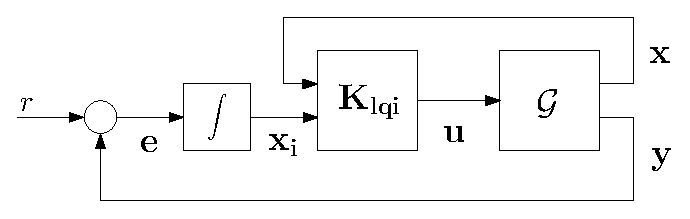
\includegraphics[width=10.5cm]{lqi}
	\caption{Closed-loop system with LQI controller for reference tracking}
	\label{fig:lqi}
	\end{center}
	\end{figure}


\subsection{$H_\infty$ Controller}
\subsubsection{$H_\infty$ Synthesis for Controller Design}
The design of the $H_\infty$ controller is based on a representation of the closed-loop system including the generalized plant $P_H$ and the controller $K_H$, shown in Fig. \ref{fig:generalized}.
	\begin{figure}[h]
	\begin{center}
	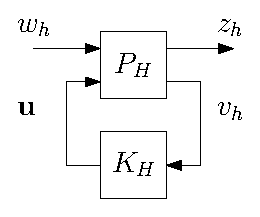
\includegraphics[width=4.5cm]{generalized}
	\caption{Control loop with generalized plant}
	\label{fig:generalized}
	\end{center}
	\end{figure}
\\\\The generalized plant $P_H$ corresponds to the system
\begin{align}
\begin{split}
\mathbf{\dot{x}} & = A\mathbf{x} + B_{w}w_{h} + B\mathbf{u},\\[5px]
z_{h} & = C_{z}\mathbf{x} + D_{zw}w_{h} + D_{zu}\mathbf{u},\\[5px]
v_{h} & = -C\mathbf{x} + D_{vw}w_{h} + D_{vu}\mathbf{u}.
\end{split}
\end{align} 
where $w_h$ are the external inputs, including command inputs, disturbances and noises; $z_h$ is a fictitious output vector used to express design specifications; and $v_h$ are the measured outputs of the system \cite{Werner2012}.
\\\\
The $H_\infty$ design procedure aims to synthesize a dynamic controller $K_H$, with input $v_h = -\mathbf{y}$ and output $\mathbf{u}$, such that the closed-loop system is stabilized and the fictitious output $z_h$ is minimized.
\\\\
The system in Fig. \ref{fig:generalized}, is rearranged for easy interpretation, in the way of Fig. \ref{fig:augmentedPlant}.
\begin{figure}[h]
	\begin{center}
	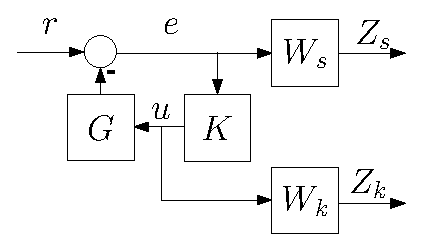
\includegraphics[width=6.5cm]{augmentedPlant.eps}
	\caption{Generalized plant with the weighting filters $W_s$ and $W_k$.}
	\label{fig:augmentedPlant}
	\end{center}
	\end{figure}	
\\In Fig. \ref{fig:augmentedPlant}, $\mathcal{G}$ represents the quadrotor dynamics; $K_H$ the controller; $r$ is the system reference; $\mathbf{e}$ is the error; $\mathbf{u}$ is the control input; $z_{h} = \begin{bmatrix}
Z_s & Z_k
\end{bmatrix}$; and $W_{s},\ W_{k}$ are weighting filters that must satisfy 
	\begin{equation}\label{eqn:hinf}
	\gamma = \left|\left|\begin{bmatrix}
	W_{s}S\\W_{k}K_{H}S
	\end{bmatrix}\right|\right|_{\infty} < 1,
	\end{equation}
\\where $S$ is the sensitivity function and $K_{H}S$ is the control sensitivity defined as
	\begin{equation}
	S = (\mathcal{I} + \mathcal{G}K_{H})^{-1},\ \ \ K_{H}S = K_{H}(\mathcal{I} + \mathcal{G}K_{H})^{-1}.
	\end{equation}
The $H_\infty$ norm is defined only for proper and stable systems, so the weighting filters must satisfy that condition. The weighting filter $W_{s}$ impose an upper bound on the sensitivity and is designed taking into account that it is desired to have integral action in the closed-loop. This ensures a zero steady-state error. On the other hand, the filter $W_k$ impose an upper bound on the control sensitivity and must have a high-pass behaviour.
\\\\
The weighting filters for the sensitivity and the control sensitivity are chosen as
\begin{align}\label{eqn:wswk}
\begin{split}
W_{s} &= \dfrac{w_{s}/M_{s}}{s + w_{s}}*\mathcal{I}_{n_{y}\times n_{y}}\ ,\\
W_{k} &= \dfrac{c_k}{M_{k}}\dfrac{s+w_{k}}{s+c_{k}w_{k}}*\mathcal{I}_{n_{u}\times n_{u}}\ ,
\end{split}
\end{align}
where $M_s$ is small constant that sets an upper bound on the sensitivity at low frequencies; and $w_s$ is a small constant that ensures that $W_s$ does not have a pole at the origin; $M_k$ is a constant that sets the upper bound on the control sensitivity at low frequencies; $w_k$ is a small constant that place the zero of $W_k$ near the origin; and $c_k$ is a large constant that place the pole of $W_k$ at a frequency above the bandwidth.
\\\\
If the resulting value of $\gamma$ is greater than one, the design procedure is iterated normalizing the weighting filters with $\gamma$.
\\\\
In this project, the synthesized optimal $H_\infty$ controllers $K_H$ are computed using the Robust Control Toolbox of MATLAB.

\subsubsection{$H_\infty$ Controller Order Reduction}
The designed $H_{\infty}$ controller $K_H$ is a dynamic model with $n_u$ outputs, $n_y$ inputs and
order $n_H = n_{x} + n_{y} + n_{u}$. To reduce the computational load that the execution of a high-order dynamic system entails, it is necessary to find a reduced order controller that behaves similarly to the full order controller $K_H$. 
\\\\
In a dynamic system, the states with small singular value energy in $\mathcal{W}_{c}$ show a weak response to a control input, while states with small singular value energy in $\mathcal{W}_{o}$ have weak influence on the observed output. In order to check which states of $K_H$ have little influence both in terms of controllability and observability, the singular values of the Hankel matrix
\begin{equation}
H_{k} = \mathcal{O_{K_H}}\mathcal{C_{K_H}},
\end{equation}
are analysed. The matrices $\mathcal{C_{K_H}}$ and $\mathcal{O_{K_H}}$ represent the controllability and observability matrices of the system $K_H$, respectively. A Hankel singular value (HSV) with small energy indicates that a state has little influence both in terms of controllability and observability.
\\\\
If $\hat{K}_{H}=(\hat{A}_H,\ \hat{B}_H,\ \hat{C}_H,\ \hat{D}_H)$ is the balanced realization of $K_H$ with $n_H$ state variables, and we have $n_h$ significant states, so the last $n_{H}-n_{h}$ HSVs are small enough to be neglected without modifying the system dynamics \cite{Skogestad2005}. 

\section{Design and Simulation of Controllers}
\label{sec:controldesign}
This section shows the specific design for the LQI and $H_\infty$ controllers in each of the quadrotor flight modes. Based on what is described on Section \ref{sec:controlstrategies}, the dynamic model for each flight mode is set. Then, the controllers are designed and simulated in order to check their proper operation.
\subsection{Stabilize Mode}
In stabilize mode, the dynamics related to the position of the quadrotor are neglected. Thus, the only $DoF$ that are automatically controlled are $\psi$, $\theta$, and $\phi$.
\subsubsection{Dynamic Model}
The dynamic model exposed in \ref{sec:linearized}, is reduced to a sixth order dynamic system ($n_x = 6$) with  three outputs ($n_y = 3$), where
\begin{align}
\begin{split}
\mathbf{x} = & \begin{bmatrix}
\psi & \dot{\psi} & \theta & \dot{\theta} & \phi & \dot{\phi}
\end{bmatrix}^{T},\\[15px]
\mathbf{y} = & \begin{bmatrix}
\psi & \theta & \phi
\end{bmatrix}^{T}.
\end{split}
\end{align}
The linear state-space representation (\ref{ec:statespace}) for the dynamics related to the stabilize mode is defined by the matrices
\begin{align}
\begin{split}
A = & 
\begin{bmatrix}
0 & 1 & 0 & 0 & 0 & 0 \\[2px]
0 & 0 & 0 & 0 & 0 & 0 \\[2px]
0 & 0 & 0 & 1 & 0 & 0 \\[2px]
0 & 0 & 0 & 0 & 0 & 0 \\[2px]
0 & 0 & 0 & 0 & 0 & 1 \\[2px]
0 & 0 & 0 & 0 & 0 & 0
\end{bmatrix}, \\[10px]
B = & 
\begin{bmatrix}
0 & 0 & 0 & 0 & 0 & 0\\[5px]
0 & \dfrac{1}{J_{zz}} & 0 & 0 & 0 & 0\\[5px]
0 & 0 & 0 & \dfrac{1}{J_{yy}} & 0 & 0\\[5px]
0 & 0 & 0 & 0 & 0 & \dfrac{1}{J_{xx}}
\end{bmatrix}^{T}.\\[10px]
C = & 
\begin{bmatrix}
1 & 0 & 0 & 0 & 0 & 0 \\[2px]
0 & 0 & 1 & 0 & 0 & 0 \\[2px]
0 & 0 & 0 & 0 & 1 & 0
\end{bmatrix}, \\[10px]
D = &\ \mathbf{0_{3\times 4}}.
\end{split}
\end{align}
Both the controllability matrix $\mathcal{C_G}$ and observability matrix $\mathcal{O_G}$, have full rank ($rank(\mathcal{C_G}) = rank(\mathcal{O_G}) = 6$), and therefore the system is controllable and observable.

\subsubsection{LQI Controller}
The design of the LQI controller is done using the penalization matrices $\mathcal{Q}$ and $\mathcal{R}$, that modify the cost function (\ref{eqn:cost}). Both matrices are set as diagonal matrices, so that there is only one parameter in the matrix affecting each state or input. The matrix $\mathcal{Q}$ must be a $9\times 9$ matrix, since the size of $\mathbf{x_{lqi}}$ is $n_x + n_y$. Similarly, $\mathcal{R}$ must have four components in its diagonal, inasmuch as the number of inputs $n_u$ remains four.
In \cite{Alsharif2017a}, the author suggests the matrices
\begin{align}
\label{eqn:QR_stabilize}
\begin{split}
\mathcal{Q} & = \mathcal{I}_{9 \times 9}\begin{bmatrix}
1 & 0.1 & 1 & 0.1 & 1 & 0.1 & 10 & 40 & 40
\end{bmatrix}^{T},\\
\mathcal{R} & = \mathcal{I}_{4 \times 4}\begin{bmatrix}
3 & 3 & 3 & 3
\end{bmatrix}^{T},
\end{split}
\end{align}
where the system outputs $\mathbf{y}$ have greater penalty than their derivatives ($\dot{\psi}$, $\dot{\theta}$, $\dot{\phi}$); $\mathbf{x_{lqi}}$ have greater penalties than $\mathbf{x}$; and the input vector $\mathbf{u}$ is slightly more penalized than $\mathbf{x}$. If the penalty of $\mathbf{x_{lqi}}$ is small, the response of the system will tend to be slow. On the other hand, if the penalty of $\mathbf{x_{lqi}}$ is very high, the controller will overcompensate the system.
\\\\
Based on the penalization matrices from (\ref{eqn:QR_stabilize}), the feedback gain matrix $\mathbf{K_{lqi}}$ is calculated. The closed-loop response of the system shown in Fig. \ref{fig:lqi} is simulated using MATLAB, and is shown in Fig. \ref{fig:stabilize_lqi}.
\begin{figure}[h]
\begin{subfigure}{.5\linewidth}
\centering
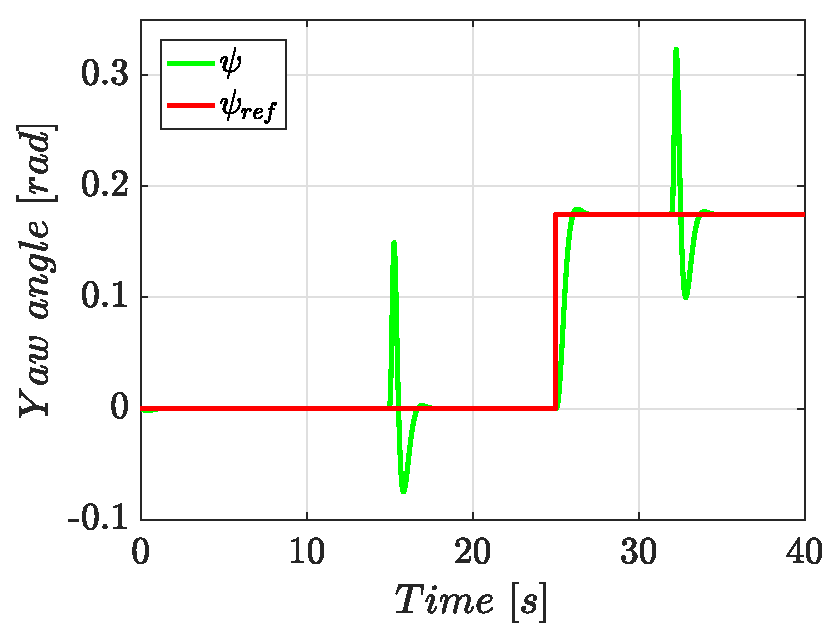
\includegraphics[width=7.0cm]{stabilize_psi_lqi}
\caption{Yaw angle response}
\label{fig:stabilize_psi_lqi}
\end{subfigure}%
\begin{subfigure}{.5\linewidth}
\centering
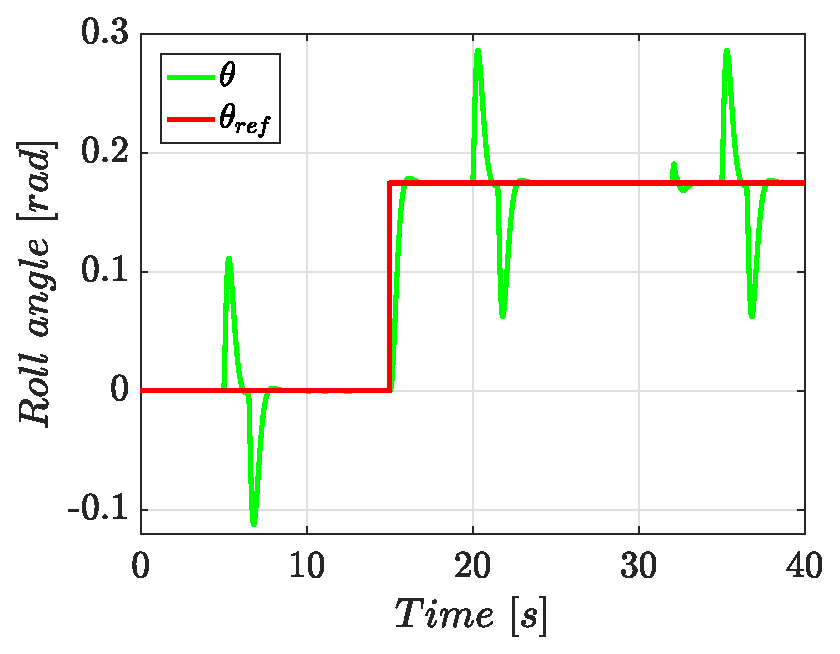
\includegraphics[width=7.0cm]{stabilize_theta_lqi}
\caption{Roll angle response}
\label{fig:stabilize_theta_lqi}
\end{subfigure}\\[1ex]
\begin{subfigure}{\linewidth}
\centering
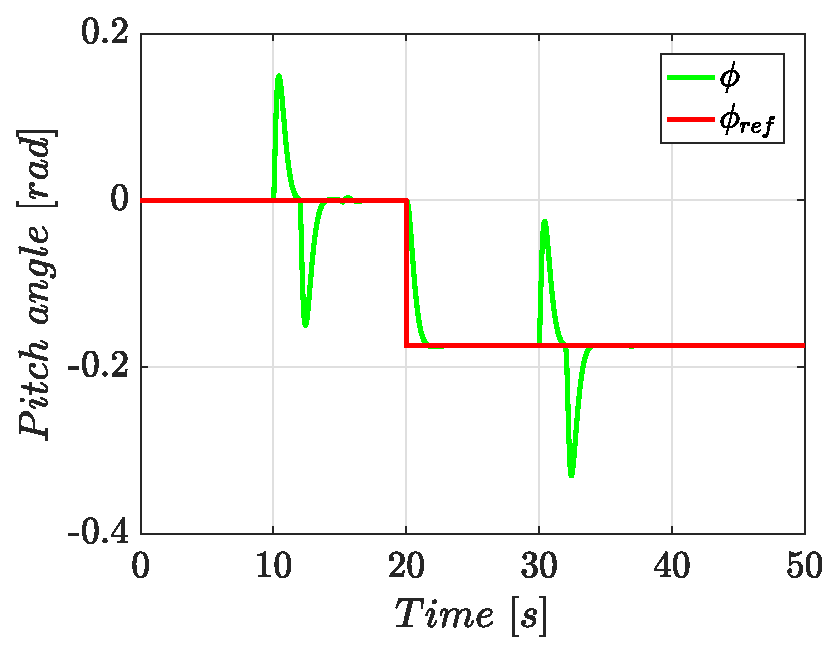
\includegraphics[width=7.0cm]{stabilize_phi_lqi}
\caption{Pitch angle response}
\label{fig:stabilize_phi_lqi}
\end{subfigure}
\caption{Simulated closed-loop response of stabilize mode controlled by a LQI controller}
\label{fig:stabilize_lqi}
\end{figure}
\\Here, the system shows responses with a setting time of less than $1.5\ s$ and overshoot of less than $5$ \%.
\subsubsection{$H_\infty$ Controller}
The design of the $H_\infty$ controller is based on the weighting filters $W_s$ and $W_k$, which are set so equation (\ref{eqn:hinf}) is satisfied.\\\\
In the case of the stabilize mode, the filters are set as 
\begin{align}
\begin{split}
W_{s} &= \dfrac{(22\cdot10^{-7})/(10^{-4})}{s + (22\cdot10^{-7})}*\mathcal{I}_{3\times 3}\ ,\\[5px]
W_{k} &= \dfrac{10^{3}}{20}\dfrac{s+50}{s+(10^{3}\cdot 50)}*\mathcal{I}_{4\times 4}\ ,
\end{split}
\end{align}
with which $\gamma = 0.0150$ was obtained. Since the $\gamma$ value is very far from $1$, the filters are normalized with $\gamma$ as
\begin{align}
\begin{split}
W_{s} &= \dfrac{1}{\gamma} W_{s},\\[5px]
W_{k} &= \dfrac{1}{\gamma} W_{k},
\end{split}
\end{align}
after which $\gamma$ is recalculated, obtaining a value of $\gamma = 0.8542 $. The filters $W_s$ and $W_k$  effectively set an upper bound for sensitivity $S$ and the control sensitivity $K_{H}S$, as shown in Fig. \ref{fig:sv_stabilize_hinf}.
\begin{figure}[h]
\begin{center}
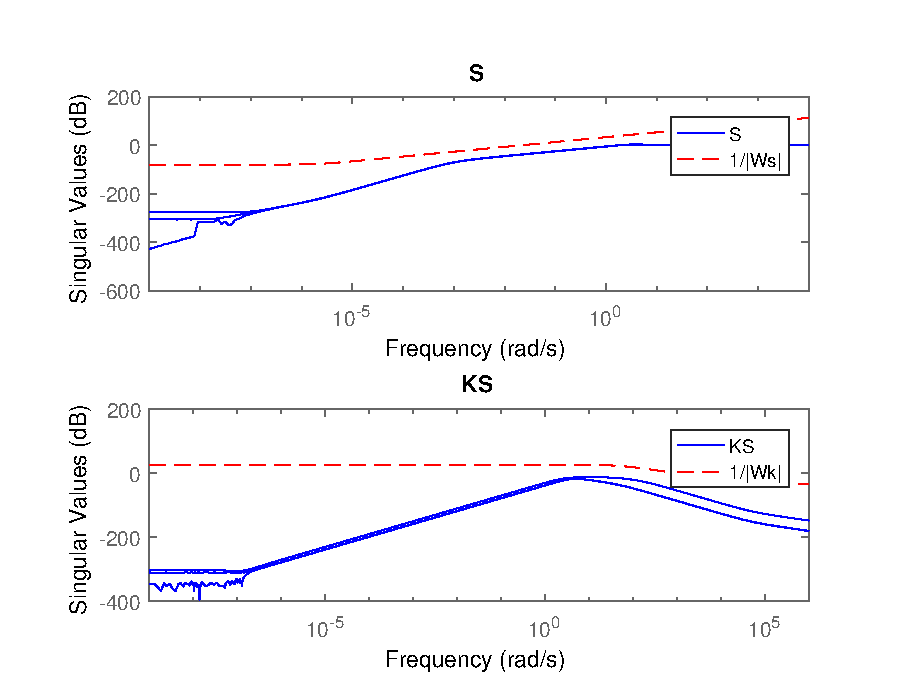
\includegraphics[width=10.3cm]{sv_stabilize_hinf}  
\caption{Upper bounded singular values of $S$ and $K_{H}S$ in stabilize mode} 
\label{fig:sv_stabilize_hinf}
\end{center}
\end{figure}
\\The computed dynamic controller $K_H$ is a $13^{th}$ order system. However, it is possible to find an equivalent system of lower order as seen in Section \ref{sec:controlstrategies}.
The energy of the HSV of $K_H$, is shown in Fig. \ref{fig:hsv_stabilize_h}.
\begin{figure}[h]
\begin{center}
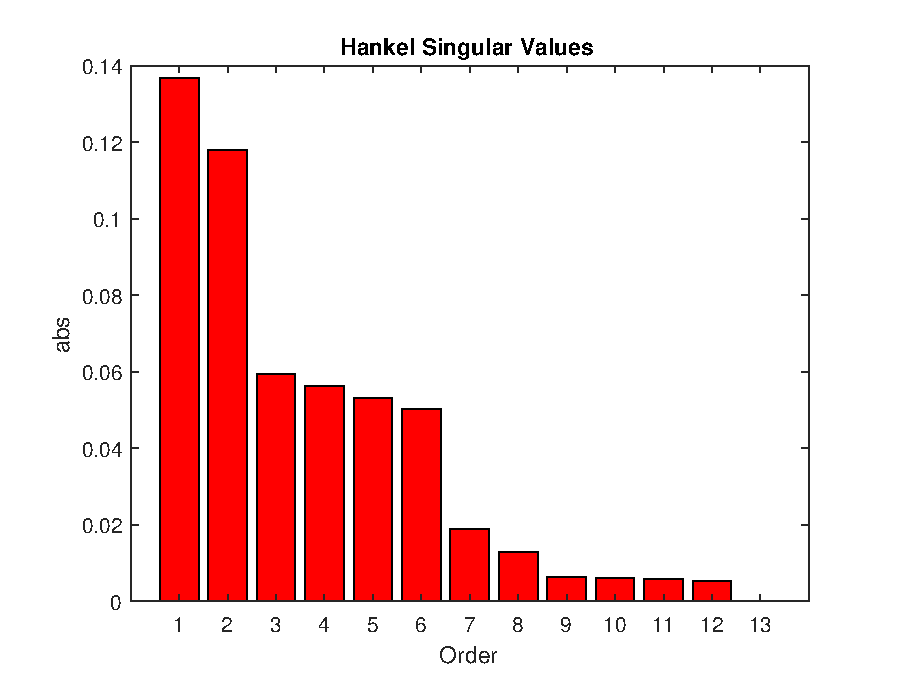
\includegraphics[width=10.8cm]{hsv_stabilize_h}  
\caption{HSV energy histogram of $K_H$ in stabilize mode} 
\label{fig:hsv_stabilize_h}
\end{center}
\end{figure}
\\\\
As shown in Fig. \ref{fig:hsv_stabilize_h}, the last ordered state of the balanced realization of $K_H$, has unnoticeable energy when it is plotted; that means that this state can be truncated from the controller without modifying its dynamics. Thus, the reduced order controller $K_{H}^{*}$ is a $12^{th}$ order system.
\\\\
Once, the optimal $H_\infty$ controller $K_{H}^{*}$ is synthesized using MATLAB, its performance is simulated. For the simulation, the system is subjected to the same disturbances and reference changes set in the LQI simulation. The simulation response is shown in Fig. \ref{fig:stabilize_h}.
\begin{figure}[h]
\begin{subfigure}{.5\linewidth}
\centering
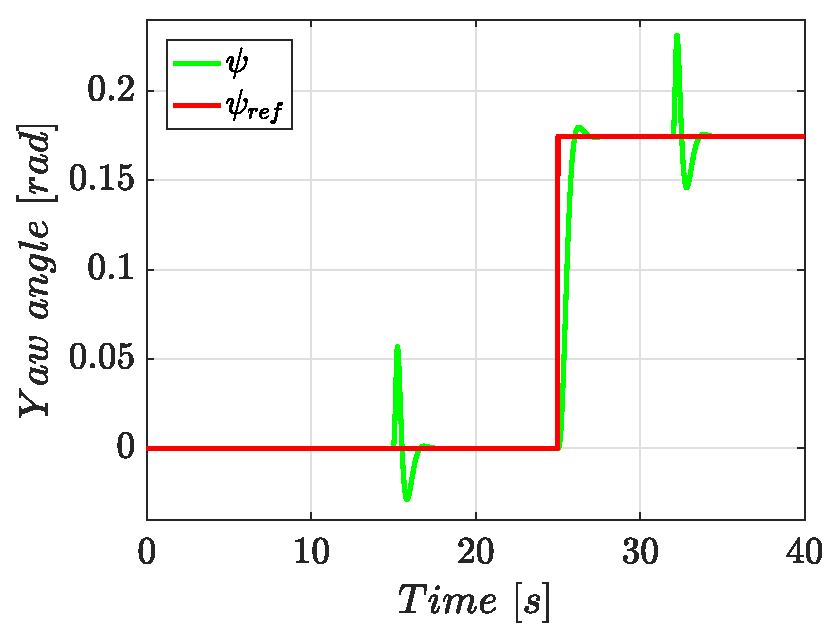
\includegraphics[width=7.0cm]{stabilize_psi_h}
\caption{Yaw angle response}
\label{fig:stabilize_psi_h}
\end{subfigure}%
\begin{subfigure}{.5\linewidth}
\centering
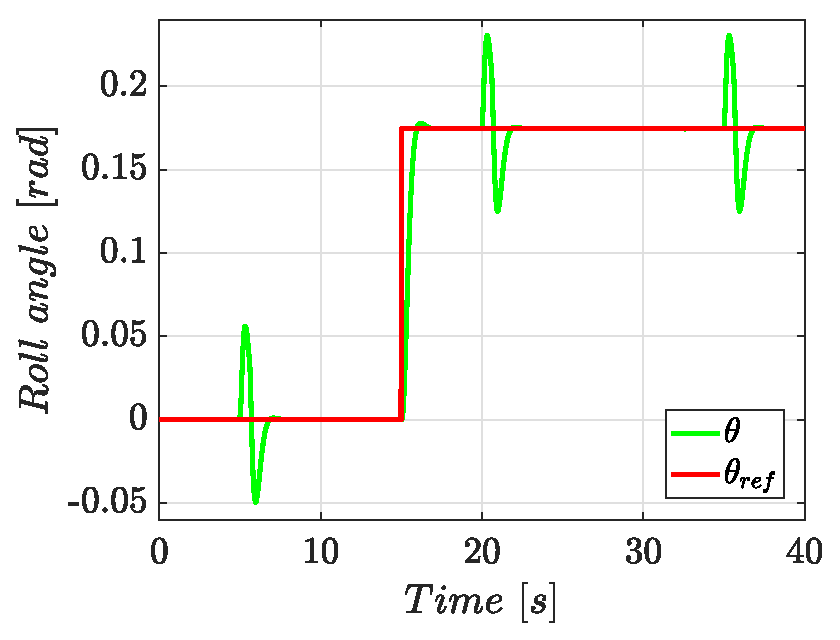
\includegraphics[width=7.0cm]{stabilize_theta_h}
\caption{Roll angle response}
\label{fig:stabilize_theta_h}
\end{subfigure}\\[1ex]
\begin{subfigure}{\linewidth}
\centering
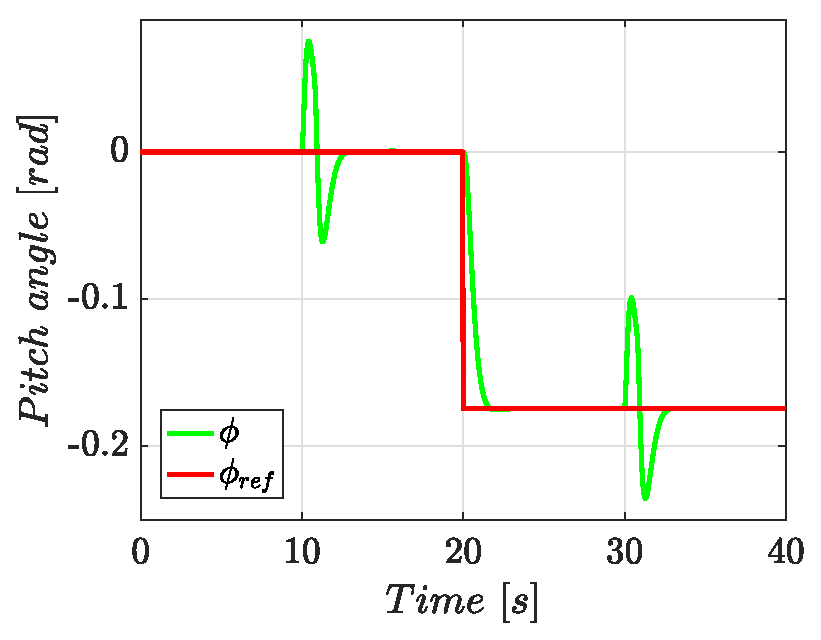
\includegraphics[width=7.0cm]{stabilize_phi_h}
\caption{Pitch angle response}
\label{fig:stabilize_psi_h}
\end{subfigure}
\caption{Simulated closed-loop response of stabilize mode controlled by a $H_\infty$ controller}
\label{fig:stabilize_h}
\end{figure}
\\\\For the $H_\infty$ controller designed for the quadrotor stabilize mode, the closed-loop performance is improved when compared to the LQI controller. The designed $K_H^{*}$ controller achieves to get responses with less than $1.1\ s$ of setting time and $3$ \% overshoot.

\subsection{Altitude Hold Mode}
This mode adds the flight altitude of the quadrotor, represented by the variable $z$, to the quadrotor controlled $DoF$. Hence, it neglects the dynamics related to the $x$ and $y$ position.
\subsubsection{Dynamic Model}
The altitude hold mode, is represented by a dynamic model of $8^{th}$ order, which states and outputs vectors are
\begin{align}
\begin{split}
\mathbf{x} = & \begin{bmatrix}
z & \dot{z} & \psi & \dot{\psi} & \theta & \dot{\theta} & \phi & \dot{\phi}
\end{bmatrix}^{T},\\[15px]
\mathbf{y} = & \begin{bmatrix}
z & \psi & \theta & \phi
\end{bmatrix}^{T}.
\end{split}
\end{align}
This dynamic system, is represented by the matrices
\begin{align}
\begin{split}
A = & 
\begin{bmatrix}
0 & 1 & 0 & 0 & 0 & 0 & 0 & 0\\[2px]
0 & 0 & 0 & 0 & 0 & 0 & 0 & 0\\[2px]
0 & 0 & 0 & 1 & 0 & 0 & 0 & 0\\[2px]
0 & 0 & 0 & 0 & 0 & 0 & 0 & 0\\[2px]
0 & 0 & 0 & 0 & 0 & 1 & 0 & 0\\[2px]
0 & 0 & 0 & 0 & 0 & 0 & 0 & 0\\[2px]
0 & 0 & 0 & 0 & 0 & 0 & 0 & 1\\[2px]
0 & 0 & 0 & 0 & 0 & 0 & 0 & 0
\end{bmatrix}, \\[5px]
B = & 
\begin{bmatrix}
0 & \dfrac{1}{m} & 0 & 0 & 0 & 0 & 0 & 0\\[5px]
0 & 0 & 0 & \dfrac{1}{J_{zz}} & 0 & 0 & 0 & 0\\[5px]
0 & 0 & 0 & 0 & 0 & \dfrac{1}{J_{yy}} & 0 & 0\\[5px]
0 & 0 & 0 & 0 & 0 & 0 & 0 & \dfrac{1}{J_{xx}}
\end{bmatrix}^{T}, \\[5px]
C = & 
\begin{bmatrix}
1 & 0 & 0 & 0 & 0 & 0 & 0 & 0 \\[2px]
0 & 0 & 1 & 0 & 0 & 0 & 0 & 0 \\[2px]
0 & 0 & 0 & 0 & 1 & 0 & 0 & 0 \\[2px]
0 & 0 & 0 & 0 & 0 & 0 & 1 & 0 
\end{bmatrix}, \\[5px]
D = &\ \mathbf{0_{4\times 4}}.
\end{split}
\end{align}
The controllability and observability features of the system are checked using the matrices $\mathcal{C_G}$ and $\mathcal{O_G}$. In the altitude hold dynamic model, both matrices have a $rank$ of $8$, which means that the system is controllable and observable.
\\\\
\subsubsection{LQI Controller}
For the altitude hold mode, the penalization matrices $\mathcal{Q}$ and $\mathcal{R}$ are set as
\begin{align}
\label{eqn:QR_althold}
\begin{split}
\mathcal{Q} & = \mathcal{I}_{12 \times 12}\begin{bmatrix}
1 & 0.1 & 1 & 0.1 & 1 & 0.1 & 1 & 0.1 & 10 & 10 & 40 & 40
\end{bmatrix}^{T},\\
\mathcal{R} & = \mathcal{I}_{4 \times 4}\begin{bmatrix}
3 & 3 & 3 & 3
\end{bmatrix}^{T},
\end{split}
\end{align}
so that the state $z$ has the same penalization as the other outputs, while the penalization of the unmeasured states remains being lower. The integral error of the quadrotor altitude is penalized the same way as the error of yaw, with a not so big penalization, as the pitch and roll dynamics must be prioritized.
\begin{figure}[h]
\begin{subfigure}{.5\linewidth}
\centering
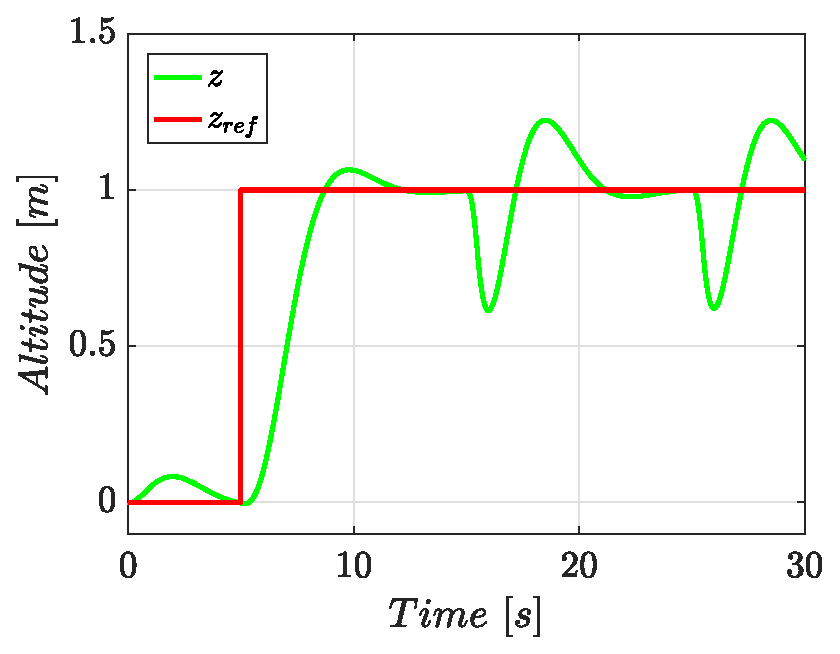
\includegraphics[width=7.0cm]{althold_z_lqi}
\caption{$z$ position response}
\label{fig:althold_z_lqi}
\end{subfigure}%
\begin{subfigure}{.5\linewidth}
\centering
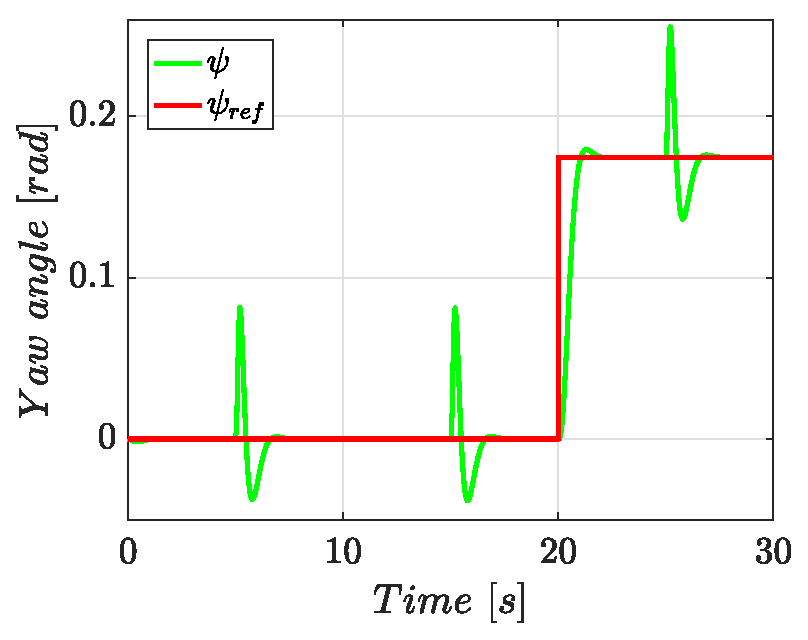
\includegraphics[width=7.0cm]{althold_psi_lqi}
\caption{Yaw angle response}
\label{fig:althold_psi_lqi}
\end{subfigure}\\[1ex]
\begin{subfigure}{0.5\linewidth}
\centering
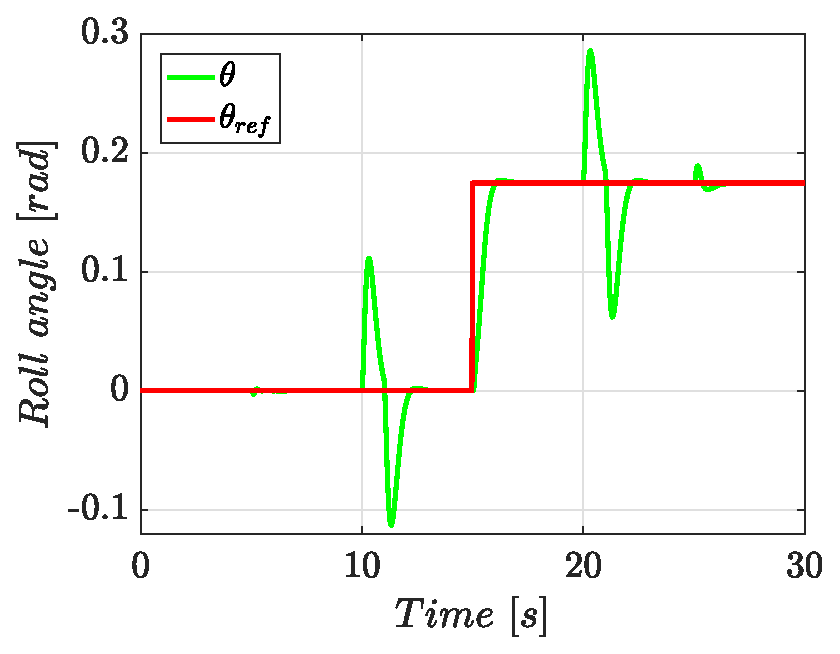
\includegraphics[width=7.0cm]{althold_theta_lqi}
\caption{Roll angle response}
\label{fig:althold_theta_lqi}
\end{subfigure}
\begin{subfigure}{0.5\linewidth}
\centering
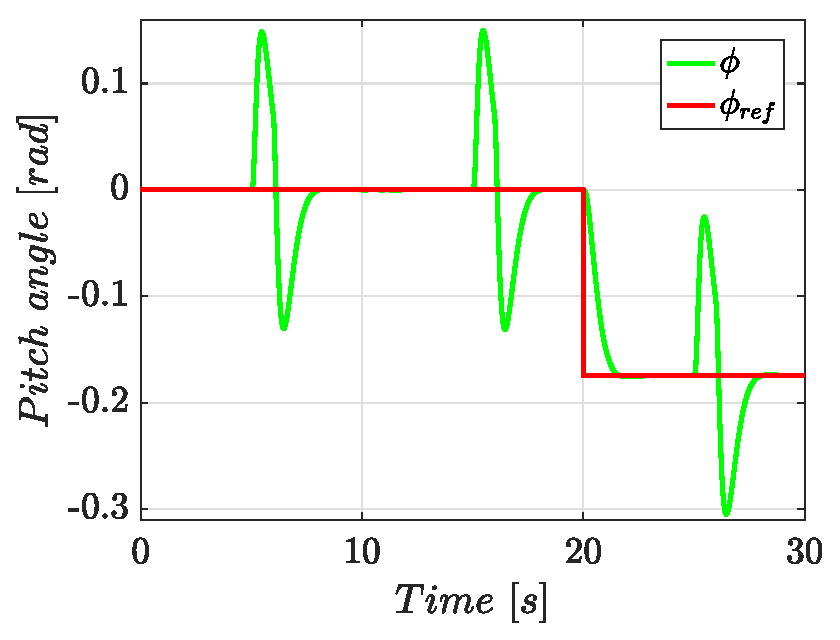
\includegraphics[width=7.0cm]{althold_phi_lqi}
\caption{Pitch angle response}
\label{fig:althold_phi_lqi}
\end{subfigure}
\caption{Simulated closed-loop response of altitude hold mode controlled by a LQI controller}
\label{fig:althold_lqi}
\end{figure}
\\
In Fig. \ref{fig:althold_lqi}, the closed-loop response of the system $\mathcal{G}_k$ in altitude hold mode with LQI control, is shown. Here, the altitude has a response with a setting time of $11.5\ s$ and an overshoot of $6$ \%. The attitude response remains the same as it is in the stabilize mode due to the use of the same penalties for the corresponding states and inputs. 

\subsubsection{$H_\infty$ Controller}
In altitude hold mode, the weighting filters which satisfy $\gamma < 1$ are
\begin{align}
\begin{split}
W_{s} &= \dfrac{(10^{-4})/(10^{-4})}{s + (10^{-4})}*\mathcal{I}_{4\times 4}\ ,\\[5px]
W_{k} &= \dfrac{10^{3}}{20}\dfrac{s+20}{s+(10^{3}\cdot 20)}*\mathcal{I}_{4\times 4}.
\end{split}
\end{align}
In this case, $\gamma = 0.5976$, forcing to iterate after normalizing the filters. After one iteration, the value of $\gamma$ is $0.9939$. The bounding of the $S$ and $K_{H}S$ functions, is shown in Fig. \ref{fig:sv_althold_hinf}
\begin{figure}[h]
\begin{center}
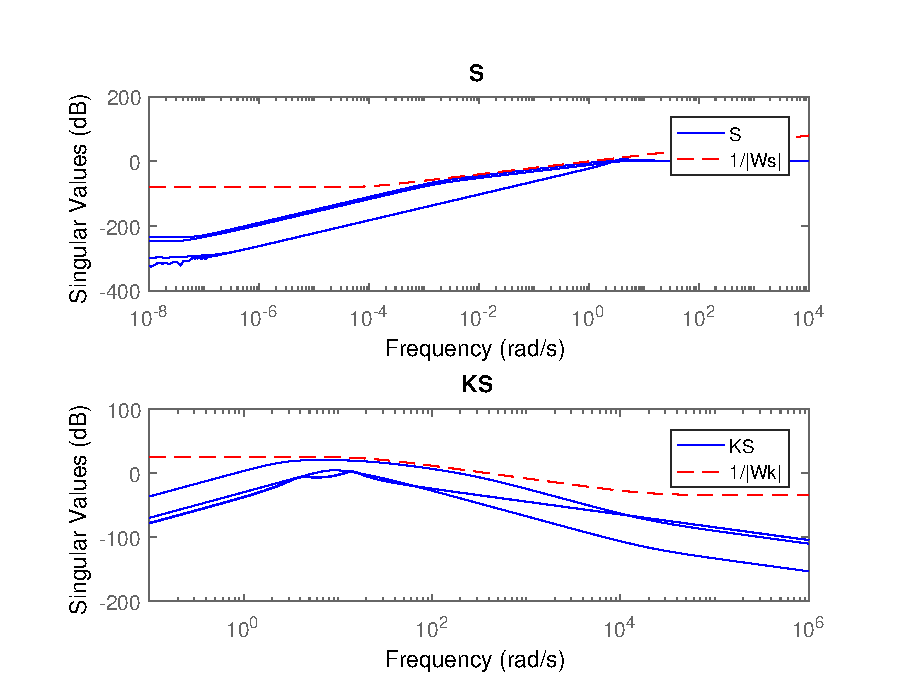
\includegraphics[width=10.3cm]{sv_althold_hinf}  
\caption{Upper bounded singular values of $S$ and $K_{H}S$ in altitude hold mode} 
\label{fig:sv_althold_hinf}
\end{center}
\end{figure}
\\\\As the dynamic model for altitude hold is a $8^{th}$ order system with $4$ inputs and $4$ outputs, the resulting $H_\infty$ controller is a $16^{th}$ dynamic system.
\begin{figure}[h]
\begin{center}
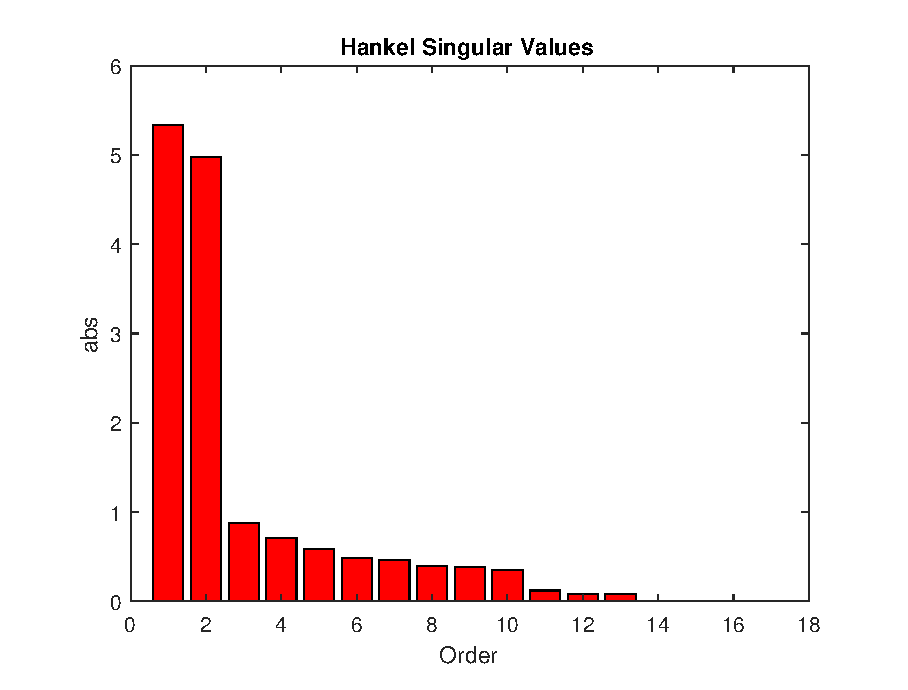
\includegraphics[width=10.8cm]{hsv_althold_h}  
\caption{HSV energy histogram of $K_H$ in altitude hold mode} 
\label{fig:hsv_althold_h}
\end{center}
\end{figure}
\\\\The $K_H$ HSV energy, exposed in Fig. \ref{fig:hsv_althold_h}, shows that there are $13$ states of $K_H$ which are influenced in terms of controllability and observability, and make up a minimal realization $K_{H}^{*}$ of $K_H$.
\\\\
The simulated response of the designed control system (Fig. \ref{fig:althold_h}), shows an improvement in setting time and overshoot when compared to the LQI controller response in the same mode. Using the $H_\infty$ controller, the setting time for $z$ is $10.7\ s$, while the overshoot is $4.5$ \%.
 
\begin{figure}[H]
\begin{subfigure}{.5\linewidth}
\centering
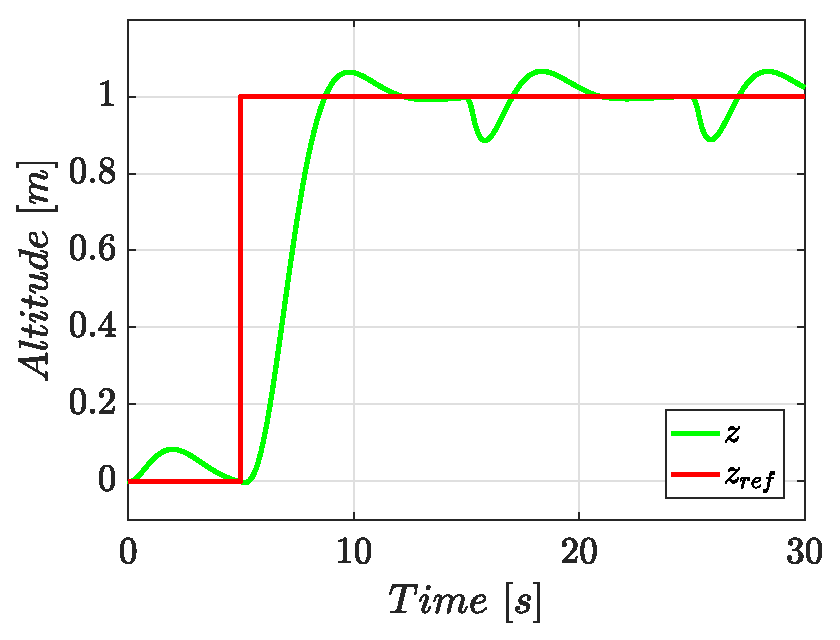
\includegraphics[width=7.0cm]{althold_z_h}
\caption{$z$ position response}
\label{fig:althold_z_h}
\end{subfigure}%
\begin{subfigure}{.5\linewidth}
\centering
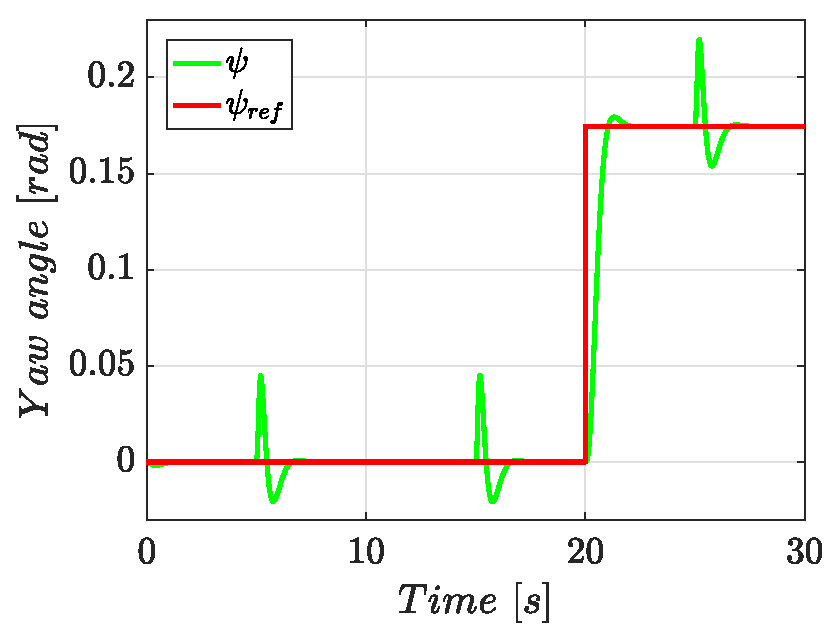
\includegraphics[width=7.0cm]{althold_psi_h}
\caption{Yaw angle response}
\label{fig:althold_psi_h}
\end{subfigure}\\[1ex]
\begin{subfigure}{0.5\linewidth}
\centering
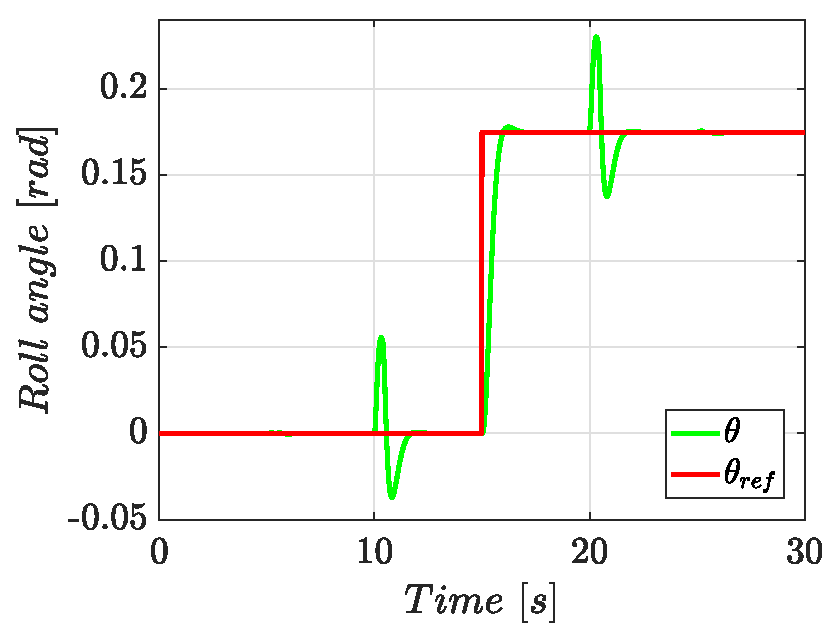
\includegraphics[width=7.0cm]{althold_theta_h}
\caption{Roll angle response}
\label{fig:althold_theta_h}
\end{subfigure}
\begin{subfigure}{0.5\linewidth}
\centering
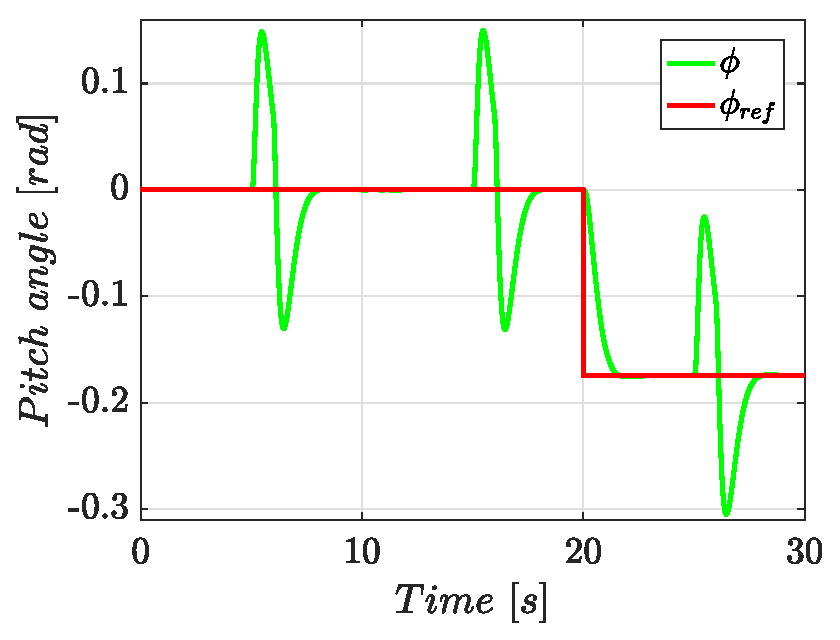
\includegraphics[width=7.0cm]{althold_phi_lqi}
\caption{Pitch angle response}
\label{fig:althold_phi_h}
\end{subfigure}
\caption{Simulated closed-loop response of altitude hold mode controlled by a $H_\infty$ controller}
\label{fig:althold_h}
\end{figure}

\subsection{GNSS-Dependent Flight Modes}
The GNSS-Dependent flight modes take into account the full states dynamics of the quadrotor. These modes include loiter, auto and RTL mode. The designed controllers can be used in any of the three mentioned modes.
\subsubsection{Dynamic Model}
The dynamic model used for the design of controllers for the GNSS-Dependent flight modes, is the full $12^{th}$ system introduced in Section \ref{sec:linearized} with all the measurable outputs available, where
\begin{align*}
\begin{split}
\mathbf{x} = & \begin{bmatrix}
x & \dot{x} & y & \dot{y} & z & \dot{z} & \psi & \dot{\psi} & \theta & \dot{\theta} & \phi & \dot{\phi}
\end{bmatrix}^{T},\\[15px]
\mathbf{y} = & \begin{bmatrix}
x & y & z & \psi & \theta & \phi
\end{bmatrix}^{T},
\end{split}
\end{align*}
\begin{align}
\begin{split}
A = & 
\begin{bmatrix}
0 & 1 & 0 & 0 & 0 & 0 & 0 & 0 & 0 & 0 & 0 & 0\\[2px]
0 & 0 & 0 & 0 & 0 & 0 & 0 & 0 & g & 0 & 0 & 0\\[2px]
0 & 0 & 0 & 1 & 0 & 0 & 0 & 0 & 0 & 0 & 0 & 0\\[2px]
0 & 0 & 0 & 0 & 0 & 0 & 0 & 0 & 0 & 0 & g & 0\\[2px]
0 & 0 & 0 & 0 & 0 & 1 & 0 & 0 & 0 & 0 & 0 & 0\\[2px]
0 & 0 & 0 & 0 & 0 & 0 & 0 & 0 & 0 & 0 & 0 & 0\\[2px]
0 & 0 & 0 & 0 & 0 & 0 & 0 & 1 & 0 & 0 & 0 & 0\\[2px]
0 & 0 & 0 & 0 & 0 & 0 & 0 & 0 & 0 & 0 & 0 & 0\\[2px]
0 & 0 & 0 & 0 & 0 & 0 & 0 & 0 & 0 & 1 & 0 & 0\\[2px]
0 & 0 & 0 & 0 & 0 & 0 & 0 & 0 & 0 & 0 & 0 & 0\\[2px]
0 & 0 & 0 & 0 & 0 & 0 & 0 & 0 & 0 & 0 & 0 & 1\\[2px]
0 & 0 & 0 & 0 & 0 & 0 & 0 & 0 & 0 & 0 & 0 & 0
\end{bmatrix}, \\[15px]
B = & 
\begin{bmatrix}
0 & 0 & 0 & 0 & 0 & \dfrac{1}{m} & 0 & 0 & 0 & 0 & 0 & 0\\[5px]
0 & 0 & 0 & 0 & 0 & 0 & 0 & \dfrac{1}{J_{zz}} & 0 & 0 & 0 & 0\\[5px]
0 & 0 & 0 & 0 & 0 & 0 & 0 & 0 & 0 & \dfrac{1}{J_{yy}} & 0 & 0\\[5px]
0 & 0 & 0 & 0 & 0 & 0 & 0 & 0 & 0 & 0 & 0 & \dfrac{1}{J_{xx}}
\end{bmatrix}^{T}.
\end{split}
\end{align}
\begin{align}
\begin{split}
C = & 
\begin{bmatrix}
1 & 0 & 0 & 0 & 0 & 0 & 0 & 0 & 0 & 0 & 0 & 0 \\[2px]
0 & 0 & 1 & 0 & 0 & 0 & 0 & 0 & 0 & 0 & 0 & 0 \\[2px]
0 & 0 & 0 & 0 & 1 & 0 & 0 & 0 & 0 & 0 & 0 & 0 \\[2px]
0 & 0 & 0 & 0 & 0 & 0 & 1 & 0 & 0 & 0 & 0 & 0 \\[2px]
0 & 0 & 0 & 0 & 0 & 0 & 0 & 0 & 1 & 0 & 0 & 0 \\[2px]
0 & 0 & 0 & 0 & 0 & 0 & 0 & 0 & 0 & 0 & 1 & 0
\end{bmatrix}, \\[15px]
D = &\ \mathbf{0_{6\times 4}}.
\end{split}
\end{align}
Verifying the controllability and observability of the system using the matrices $\mathcal{C_G}$ and $\mathcal{O_G}$, it is confirmed that these matrices have full-rank. Hence, the system is controllable and observable.

\subsubsection{LQI Controller}
Similarly to the altitude hold mode, in the GNSS-Dependent modes, the penalization matrices are
\begin{align}
\label{eqn:QR_auto}
\begin{split}
\mathcal{Q} & = \mathcal{I}_{18 \times 18}\begin{bmatrix}
1 & 0.1 & 1 & 0.1 & 1 & 0.1 & 1 & 0.1 & 1 & 0.1 & 1 & 0.1 & 10 & 10 & 10 & 10 & 40 & 40
\end{bmatrix}^{T},\\
\mathcal{R} & = \mathcal{I}_{4 \times 4}\begin{bmatrix}
3 & 3 & 3 & 3
\end{bmatrix}^{T},
\end{split}
\end{align}
where $x$ and $y$ have the same penalty as $z$, and analogously happens with $\dot{x}$, $\dot{y}$ and $\dot{z}$.
\\\\
Using MATLAB, the quadrotor controlled by the designed LQI controller, is simulated. In this simulation, the quadrotor is commanded automatically through some waypoints, which describe a square figure with constant flight altitude.
\begin{figure}[h]
	\begin{center}
	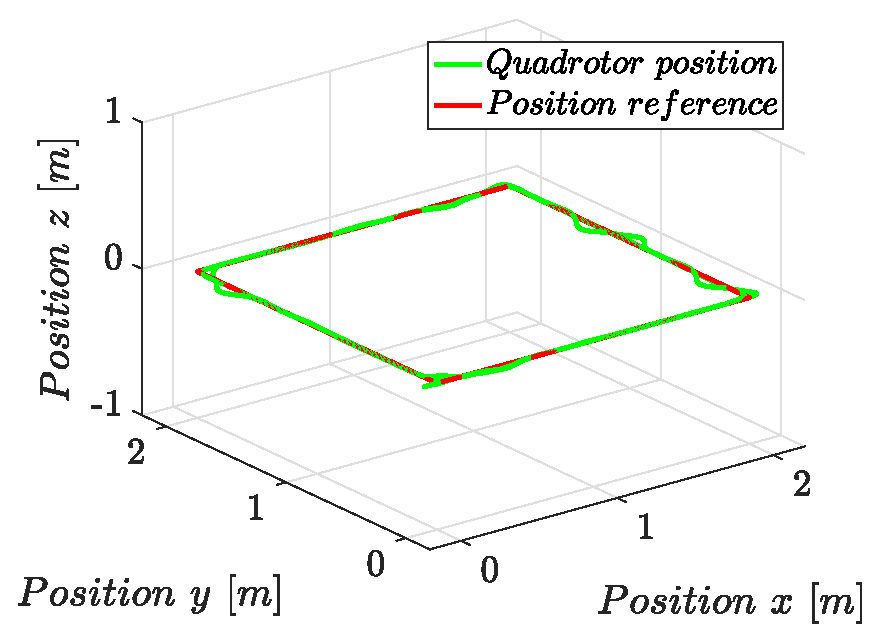
\includegraphics[width=0.7\textwidth]{auto_xyz_lqi}
	\caption{Simulated position response of the GNSS-Dependent modes with a LQI controller}
	\label{fig:auto_xyz_lqi}
	\end{center}
	\end{figure}
\begin{figure}[H]
\begin{subfigure}{.5\linewidth}
\centering
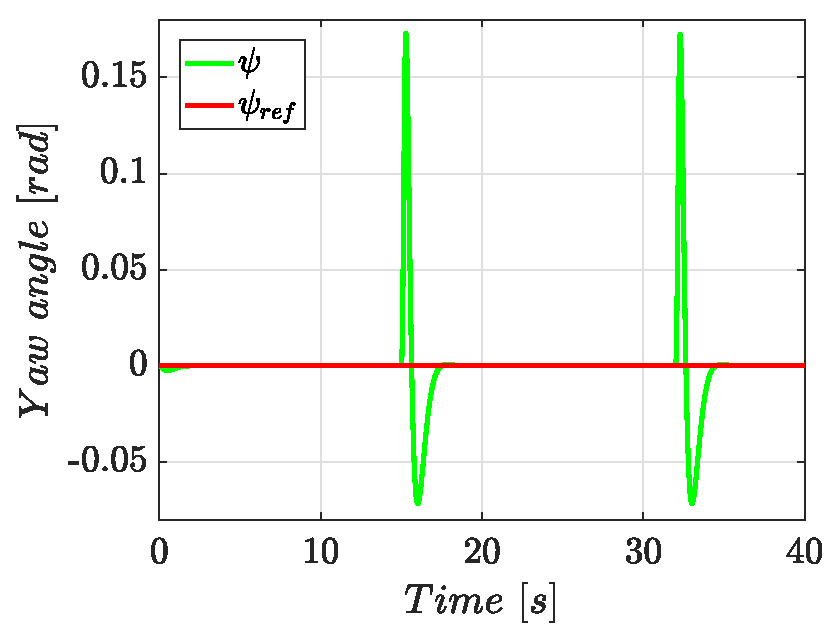
\includegraphics[width=7.0cm]{auto_psi_lqi}
\caption{Yaw angle response}
\label{fig:auto_psi_lqi}
\end{subfigure}%
\begin{subfigure}{.5\linewidth}
\centering
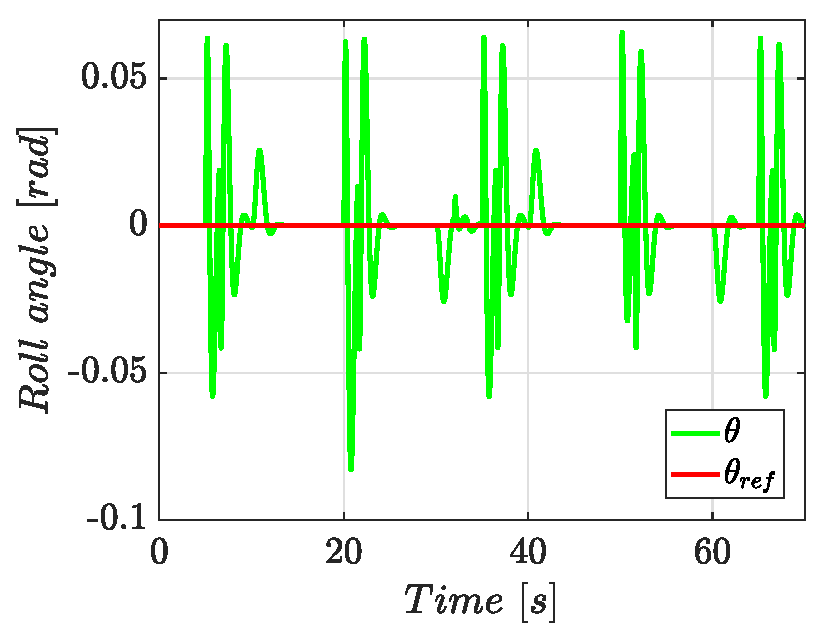
\includegraphics[width=7.0cm]{auto_theta_lqi}
\caption{Roll angle response}
\label{fig:auto_theta_lqi}
\end{subfigure}\\[1ex]
\begin{subfigure}{\linewidth}
\centering
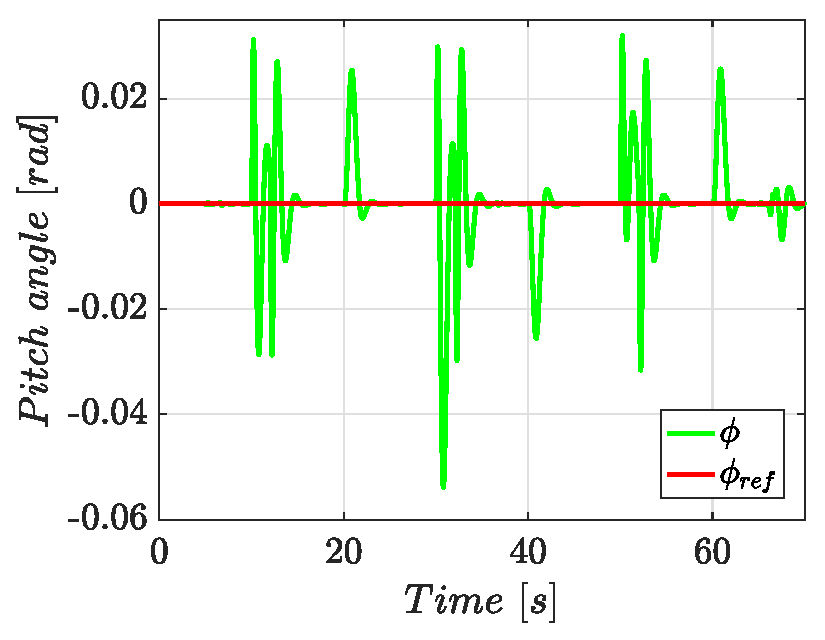
\includegraphics[width=7.0cm]{auto_phi_lqi}
\caption{Pitch angle response}
\label{fig:auto_psi_lqi}
\end{subfigure}
\caption{Simulated attitude response of the GNSS-Dependent modes with a LQI controller}
\label{fig:auto_lqi}
\end{figure}
As can be seen in Fig. \ref{fig:auto_xyz_lqi}, the quadrotor is capable of following the desired trajectory while being controlled by the LQI controller in a GNSS-Dependent mode. In addition, the quadrotor manages to recover its track in less than $3.5\ s$, after suffer the actions of disturbances that periodically simulate the force of the wind.
\subsubsection{$H_\infty$ Controller}
For the GNSS-Dependent flight modes, the weighting filter $W_s$ is now a $6\times 6$-matrix due to the existence of six output signals in $\mathbf{y}$. Thus, the weighting filters are set as
\begin{align}
\begin{split}
W_{s} &= \dfrac{(10^{-4})/(10^{-4})}{s + (10^{-4})}*\mathcal{I}_{6\times 6}\ ,\\[5px]
W_{k} &= \dfrac{10^{4}}{20}\dfrac{s+30}{s+(10^{4}\cdot 30)}*\mathcal{I}_{4\times 4}.
\end{split}
\end{align}
Wigh these weighting filters, $\gamma = 0.5976$. After one iteration, with normalized weighting filters, the $\gamma$ value becomes equal to $0.999$. Thus, the sensitivity and control sensitivity functions are closely upper bounded by the weighting filters, as shown in Fig. \ref{fig:sv_auto_hinf}.
\begin{figure}[h]
\begin{center}
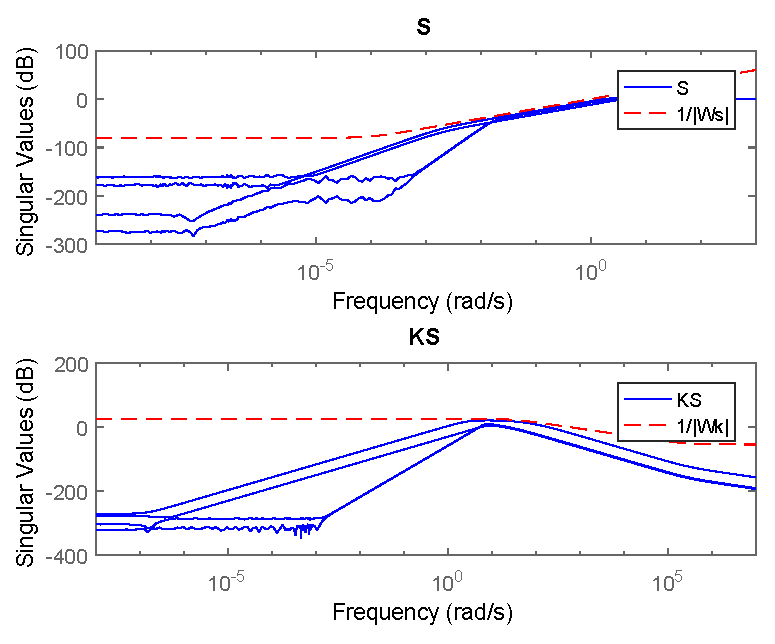
\includegraphics[width=10.3cm]{sv_auto_hinf}  
\caption{Upper bounded singular values of $S$ and $K_{H}S$ in GNSS-Dependent modes} 
\label{fig:sv_auto_hinf}
\end{center}
\end{figure}
\\\\The synthesized $H_\infty$ controller $K_H$ for the GNSS-Dependent modes has $20$ states. An equivalent controller $K_{H}^{*}$ of lower order is found, using the HSV energy shown in Fig. \ref{fig:hsv_auto_h}.
\begin{figure}[h]
\begin{center}
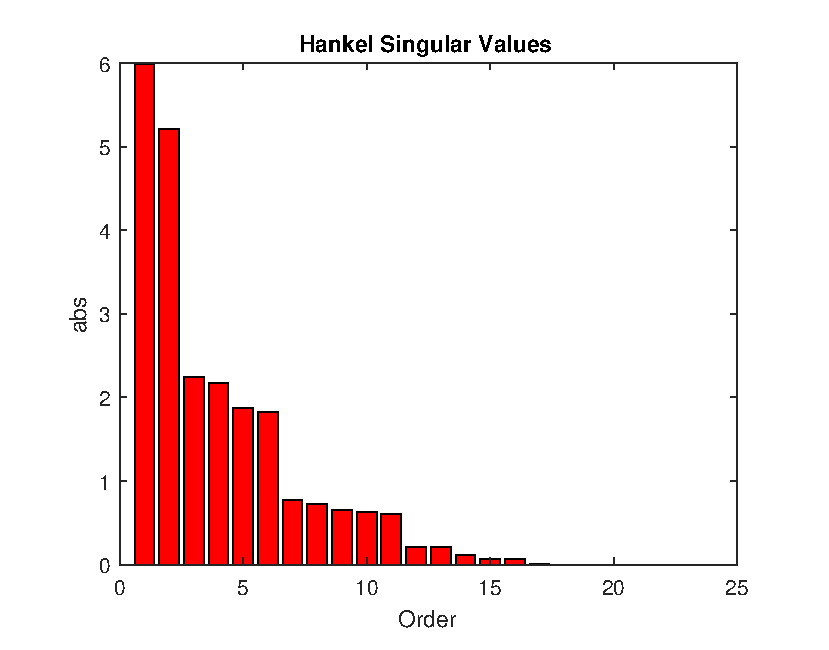
\includegraphics[width=10.8cm]{hsv_auto_h}  
\caption{HSV energy histogram of $K_H$ in GNSS-Dependent modes} 
\label{fig:hsv_auto_h}
\end{center}
\end{figure}
\\The system $K_H$ has four unnoticeable states in terms of controllability and observability, as seen in Fig. \ref{fig:hsv_auto_h}. Therefore, the reduced order controller $K_{H}^{*}$ is the subsystem of $K_H$ which includes just the $16$ noticeable states.
\\\\
The simulation of the designed $H_\infty$ controller with the quadrotor non-linear dynamics, is also developed using a reference of waypoints describing a square with sides of $2\ m$, and a constant altitude.
\begin{figure}[h]
	\begin{center}
	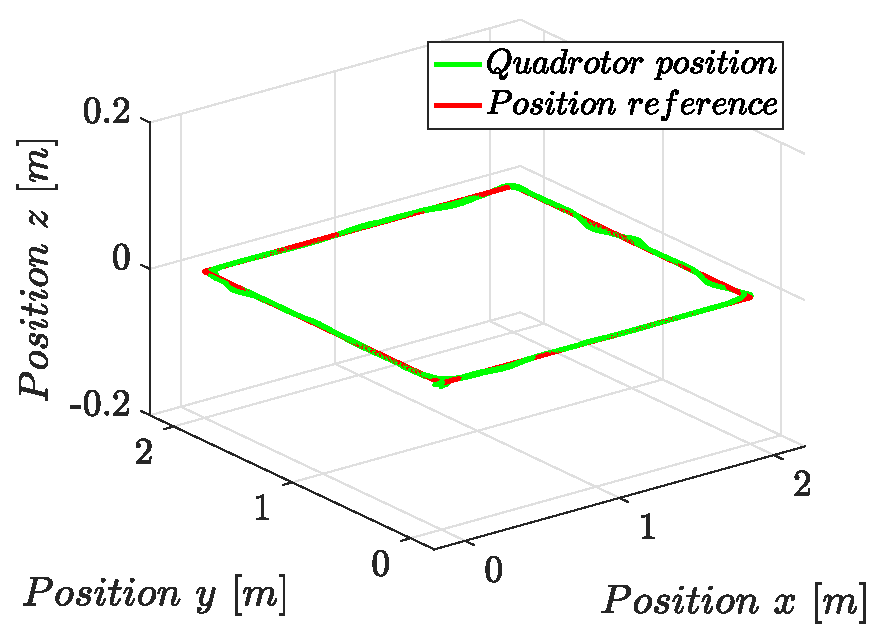
\includegraphics[width=0.7\textwidth]{auto_xyz_h}
	\caption{Simulated position response of the GNSS-Dependent modes with a $H_\infty$ controller}
	\label{fig:auto_xyz_h}
	\end{center}
	\end{figure}
\begin{figure}[H]
\begin{subfigure}{.5\linewidth}
\centering
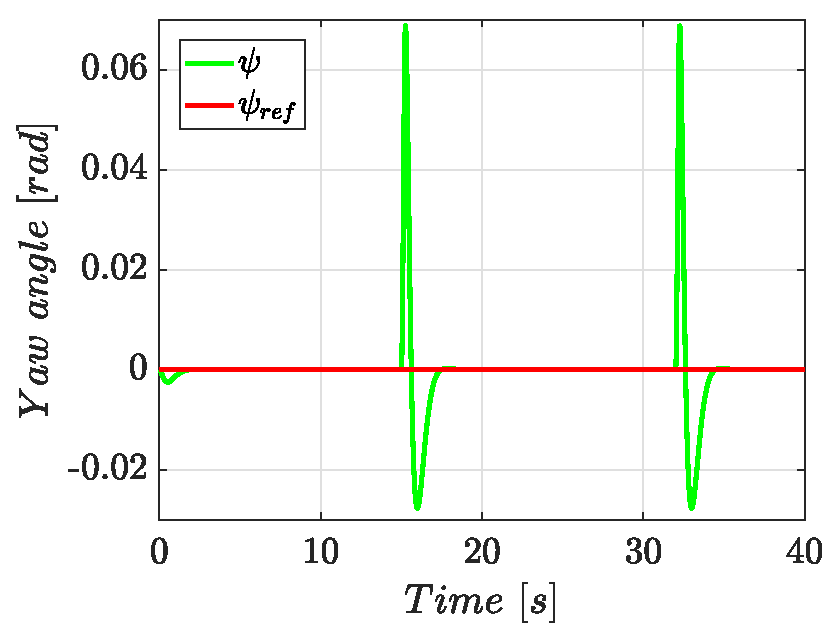
\includegraphics[width=7.0cm]{auto_psi_h}
\caption{Yaw angle response}
\label{fig:auto_psi_h}
\end{subfigure}%
\begin{subfigure}{.5\linewidth}
\centering
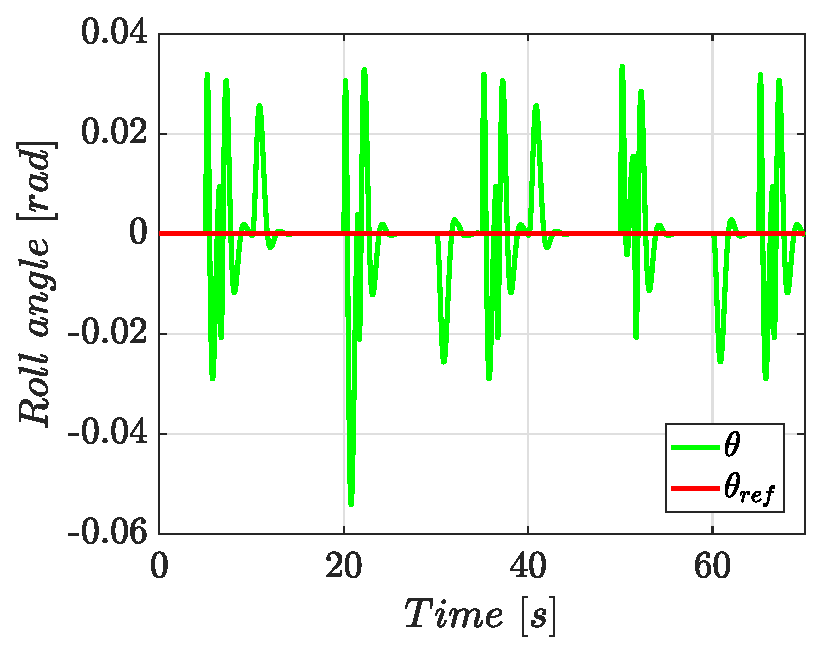
\includegraphics[width=7.0cm]{auto_theta_h}
\caption{Roll angle response}
\label{fig:auto_theta_h}
\end{subfigure}\\[1ex]
\begin{subfigure}{\linewidth}
\centering
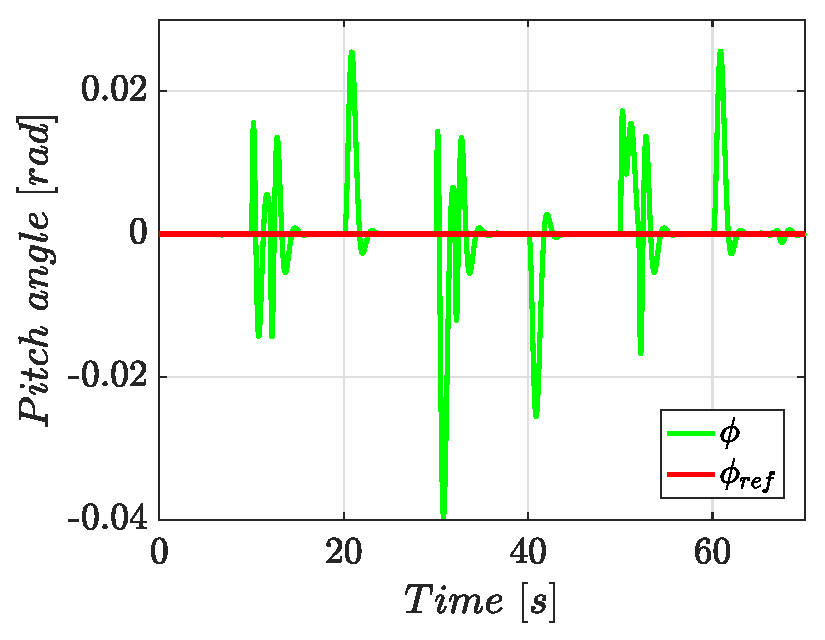
\includegraphics[width=7.0cm]{auto_phi_h}
\caption{Pitch angle response}
\label{fig:auto_psi_h}
\end{subfigure}
\caption{Simulated attitude response of the GNSS-Dependent modes with a $H_\infty$ controller}
\label{fig:auto_h}
\end{figure}
The simulated control system manages to follow the position reference, despite being affected by disturbances, as seen in Fig. \ref{fig:auto_xyz_h}. For disturbances, it shows a setting time of $2.8\ s$.

\section{State Estimation Through Kalman Filter}
\label{sec:stateestimation}
The quadrotor dynamics are sensed exclusively using the on-board smartphone sensors. These sensors have different sample frequencies and poor accuracy. On the other hand, the LQI controller needs a full-state feedback, but it is not posible to get reliable measurements of all the components in $\mathbf{x}$ in a smartphone. Hence, it is necessary to use estimation algorithms, as a Kalman filter. The principle of separation allows the design of controllers and state estimators independently.

\subsection{Attitude Estimation}
The Android API implements a Kalman filter for attitude estimation using the raw data deliverd by the smartphone accelerometer, gyroscope and magnetometer, as exposed in \cite{Astudillo2017}. Using the quaternion $Q_s$ delivered by the Rotation virtual sensor included in the Android SDK, it is obtained an absolute orientation representation with respect to the Earth frame \cite{AndSensor}, with
\begin{align}\label{eqn:rotvector}
\begin{split}
Q_{s} &= \mathrm{e}^{(\alpha/2)(u\vv{i}+v\vv{j}+w\vv{k})} \\
&= \begin{bmatrix}
\kappa_{0}\sin(\alpha / 2)\\
\kappa_{1}\sin(\alpha / 2)\\
\kappa_{2}\sin(\alpha / 2)\\
\cos(\alpha / 2)
\end{bmatrix} = \begin{bmatrix}
q_{0} \\
q_{1} \\
q_{2} \\
q_{3}
\end{bmatrix}
\end{split}
\end{align}
where $\alpha$ is the amount of degrees the quaternion is rotated around the axis $\kappa_{0}\vv{i}+\kappa_{1}\vv{j}+\kappa_{2}\vv{k}$. The rotation matrix $\mathbf{R_{b}^{w}}$ can be defined using $Q_s$ as
\begin{equation}
\label{eqn:rotbw2}
\mathbf{R_{b}^{w}} = \begin{bmatrix}
1-2(q_{2}^{2}+q_{3}^{2}) & 2(q_{1}q_{2}-q_{0}q_{3}) & 2(q_{0}q_{2}+q_{1}q_{3}) \\
2(q_{1}q_{2}-q_{0}q_{3}) & 1-2(q_{1}^{2}+q_{3}^{2}) & 2(q_{2}q_{3}+q_{0}q_{1}) \\
2(q_{1}q_{3}+q_{0}q_{2}) & 2(q_{0}q_{1}+q_{2}q_{3}) & 1-2(q_{1}^{2}+q_{2}^{2})
\end{bmatrix}.
\end{equation}
Comparing (\ref{eqn:rotbw1}) and (\ref{eqn:rotbw2}), the Euler angles ($\psi_{m}$, $\theta_m$, $\phi_m$) are then obtained from the quaternion $Q_s$ as
\begin{equation}\label{eqn:quattoeu}
\begin{bmatrix}
\psi_{m} \\
\theta_{m} \\
\phi_{m}
\end{bmatrix} =
\begin{bmatrix}
atan2(2(q_{3}q_{2} + q_{0}q{1}),1-2(q_{1}^{2} + q_{2}^{2})) \\
arcsin(2(q_{3}q_{1} - q_{2}q_{0})) \\
atan2(2(q_{3}q_{0} + q_{1}q{2}),1-2(q_{0}^{2} + q_{1}^{2})) 
\end{bmatrix}.
\end{equation}

\subsection{Position Measurement}
The smartphone used in this project, can measure its position with respect to the Earth-frame. For this task, it counts with a GNSS receiver and a barometer.
The $x_{m}$ and $y_{m}$ position measurements, with respect to the $X_W$ and $Y_W$ axes, are acquired using the GNSS receiver. 
\\\\
Each coordinates sample is initially set in an ellipsoidal representation of decimal degrees, following the WGS84 coordinate system. Then, the coordinates are converted to a bi-dimensional representation in meter units using the cartographic projection Magna-Sirgas (projection EPSG:3115).
\\\\
The altitude measurements $z_{m}$ are acquired using the barometric pressure sensor which delivers the pressure value $p_k$ in hPa units. This signal is converted to meters as
\begin{equation}\label{eqn:hbarom}
z_{m} = 44330\left(1-\frac{p_k}{p_{0}}^{1/5.255}\right)\ [m],
\end{equation}
where $p_{0}$ is the atmospheric pressure at sea level \cite{Lauszus2015}.
\\\\
The smartphone GNSS receiver and barometer were tested statically, leaving the phone in a stable position for 100 minutes, with an ambient temperature of $22\ ^{\circ}C$ and a UV index of $3$. The results of the test are shown in Fig. \ref{fig:sensorstest}.
\begin{figure}[h]
\begin{subfigure}{.5\linewidth}
\centering
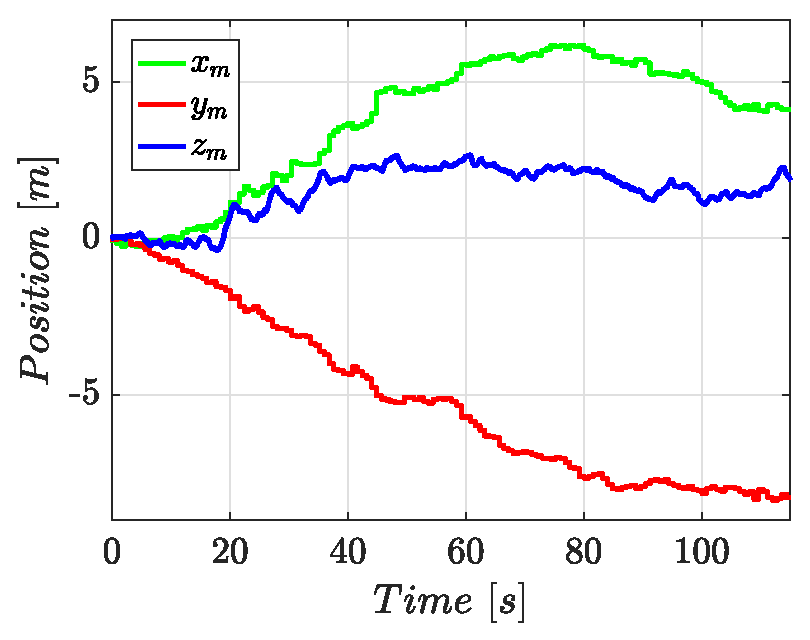
\includegraphics[width=7.0cm]{pos_test}
\caption{Position drift}
\label{fig:pos_test}
\end{subfigure}%
\begin{subfigure}{.5\linewidth}
\centering
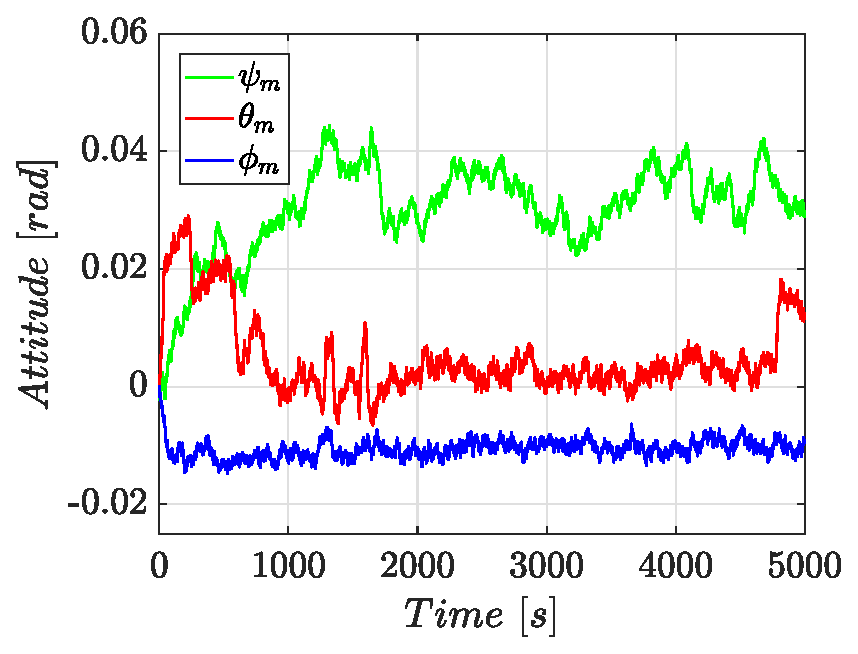
\includegraphics[width=7.0cm]{att_test}
\caption{Attitude drift}
\label{fig:att_test}
\end{subfigure}\\[1ex]
\begin{subfigure}{\linewidth}
\centering
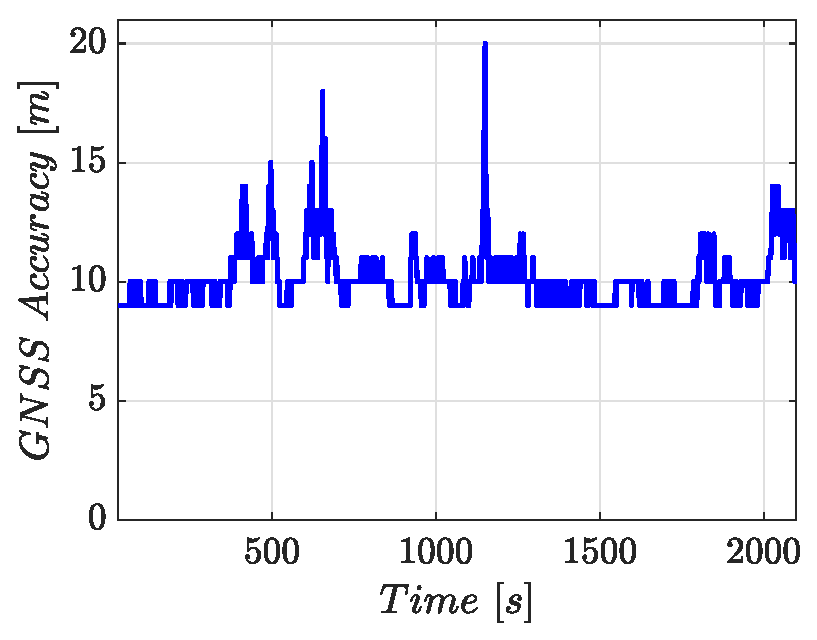
\includegraphics[width=7.0cm]{gpsacc_test}
\caption{GNSS receiver accuracy}
\label{fig:gpsacc_test}
\end{subfigure}
\caption{Static test of the smartphone GNSS receiver and barometer}
\label{fig:sensorstest}
\end{figure}
\\\\As seen in Fig. \ref{fig:pos_test}, even though the phone was kept in a static position, the $x_m$ and $y_m$ position signal received from the GNSS receiver shows a change of about $6\ m$ in both the $X_W$ and $Y_W$ directions, after just $60\ s$. The $z_m$ position, however, has sudden changes in short periods of time, but without reaching errors greater than $2.5\ m$. The attitude results, Fig. \ref{fig:att_test}, show stable signals for the three Euler angles. The $\psi_m$ and $\theta_m$ angles suffer from a drift of about $0.04$ and $-0.02\ rad$ respectively, while the initial drift suffered by $\phi_m$ is just $-0.01\ rad$.
\\\\
Despite being under a clear sky, where the smartphone could have visibility of more than six satellites of the GPS and GLONASS constellations, the GNSS accuracy value, delivered by the receiver in the smartphone, is always more than $9\ m$ as seen in Fig. \ref{fig:gpsacc_test}. 
\\\\
\subsection{State Estimation}
In order to estimate all the components of the state vector $\mathbf{x}$, a Kalman filter is designed. The Kalman filter is an iterative algorithm that estimates the observable (and not measurable) states of a system, using the measurable variables, the inputs and the variances of the noises that affect the system.
\\\\
This filter is designed using the linearized dynamic model of the quadrotor from Section \ref{sec:linearized}, where $\mathbf{x} =  \begin{bmatrix}
x & \dot{x} & y & \dot{y} & z & \dot{z} & \psi & \dot{\psi} & \theta & \dot{\theta} & \phi & \dot{\phi}
\end{bmatrix}^{T}$, and using the discretized representation $\mathcal{G}_k$.
\\\\
The algorithm starts calculating a prediction of the state $\hat{\mathbf{x}}_{k}^{-}$ and its covariance $P_{k}^{-}$ as
\begin{equation}\label{eqn:statePrognosis}
\hat{\mathbf{x}}_{k}^{-} = A_k\hat{\mathbf{x}}_{k-1}+B_k\mathbf{u},
\end{equation}
\begin{equation}\label{eqn:covariancePrognosis}
P_{k}^{-} = A_k P_{k-1} A_{k}^{T} + Q_{k},
\end{equation}
where $\hat{\mathbf{x}}_{k-1} = \hat{\mathbf{x}}(k-1)$ is the previous estimated state, $P_{k-1}$ the previous error covariance matrix and $Q_{k}$ the process variance. The state prediction is then corrected using the Kalman gain vector
\begin{align}\label{eqn:correctionKalman}
\begin{split}
K_{k} &= P^{-}_{k}H^{T}(HP^{-}_{k}H^{T} + R_k)^{-1},
\end{split}
\end{align}
and updating the state estimation $\hat{\mathbf{x}}_{k}$ and its covariance $P_{k}$, based on the measurements $\vartheta_k$ as
\begin{align}\label{eqn:correctionKalman2}
\begin{split}
\hat{\mathbf{x}}_{k} &= \hat{\mathbf{x}}^{-}_{k} + K_{k}(\vartheta_{k} - H\hat{\mathbf{x}}^{-}_{k}),\\
P_{k} &= (\mathcal{I} - K_{k}H)P^{-}_{k},
\end{split}
\end{align}
where $R_k$ is the measurement covariance matrix, $\mathcal{I}$ is the identity matrix and $H$ is the matrix that satisfies
\begin{equation}
\vartheta_k = H \mathbf{x}_k.
\end{equation}
The measurements vector $\vartheta_k$ is set as
\begin{equation}
\vartheta_k = \begin{bmatrix}
x_{m} & y_{m} & z_{m} & \psi_{m} & \theta_{m} & \phi_{m}
\end{bmatrix}^{T},
\end{equation}
so matrix $H$ is defined as
\begin{equation}\label{eqn:H}
H =\begin{bmatrix}
1 & 0 & 0 & 0 & 0 & 0 & 0 & 0 & 0 & 0 & 0 & 0\\
0 & 0 & 1 & 0 & 0 & 0 & 0 & 0 & 0 & 0 & 0 & 0\\
0 & 0 & 0 & 0 & 1 & 0 & 0 & 0 & 0 & 0 & 0 & 0\\
0 & 0 & 0 & 0 & 0 & 0 & 1 & 0 & 0 & 0 & 0 & 0\\
0 & 0 & 0 & 0 & 0 & 0 & 0 & 0 & 1 & 0 & 0 & 0\\
0 & 0 & 0 & 0 & 0 & 0 & 0 & 0 & 0 & 0 & 1 & 0
			\end{bmatrix}.
\end{equation}
This algorithm is executed once every sampling period, after which, the controller can use the vector of estimated states $\hat{\mathbf{x}}_{k}$ as feedback.



\section{Conclusions}
The control and state estimation algorithms design procedure is presented in this chapter. The concepts of system representation as a state-space model, controllability and observability, were introduced in the first part. Given the need for achieving trajectory tracking with the quadrotor, a LQR controller with integral feedback (LQI) is designed. This controller ensures zero steady-state error. Also, a controller based on the $H_\infty$ synthesis is designed. The performance of these controllers is simulated acting with the non-linear dynamic model of the quadrotor. As a result of these simulations, the $H_\infty$ controller showed a better performance when subjected to exactly the same disturbances and reference changes as the LQI controller.
Finally, due to the principle of separation, a state estimator based on a Kalman filter is designed taking into account the accuracy of the smartphone measurements.
\chapter{Implementation and Results} \label{ch:implementation}


\section{Kalman Filter for States Estimation}

\section{Linear Quadratic Regulator Results}

\subsection{Simple Translational Movements (LQR)}

\subsection{Trajectory Tracking (LQR)}

\section{H$\infty$ Regulator Results}

\subsection{Simple Translational Movements (H$\infty$)}

\subsection{Trajectory Tracking (H$\infty$)}

\addcontentsline{toc}{chapter}{Conclusions and Outlook}
\chapter*{Conclusions and Outlook \label{ch:conclusions}}
\addcontentsline{toc}{chapter}{Conclusions and Outlook}
In this thesis distributed algorithms 


\appendix


\printindex
%\glsaddall
%\printglossaries



%%% Back matter %%% 

\backmatter

\addcontentsline{toc}{chapter}{\bibname}

%\bibliographystyle{IEEEtran}	% (uses file "plain.bst")
%\bibliography{references_biblio_mas}		% expects file "myrefs.bib"
%\bibliographystyle{plainnat}
%\bibliographystyle{abbrvnat}
\bibliographystyle{unsrtnat}
\bibliography{bib/er_biblio}
%\bibliography{{./references/dokbiblio.bib/}}

\cleardoublepage
\addcontentsline{toc}{chapter}{Publications}
\chapter*{Publications} \label{publications}

\
A. Astudillo, P. Muñoz, F. Alvarez and E. Rosero, “Altitude and attitude cascade controller for a smartphone-based quadcopter,” in \textit{2017 International Conference on Unmanned Aircraft Systems (ICUAS)}. IEEE, jun 2017, pp. 1447–1454. [Online]. Available: \url{http://ieeexplore.ieee.org/document/7991400/}
\\\\
A. Astudillo, B. Bacca and E. Rosero, “Optimal and robust controllers design for a smartphone-based quadrotor,” in \textit{2017 IEEE 3rd Colombian Conference on Automatic Control (CCAC)}.
\






\end{document}


